\documentclass[reprint,aps,pra,floatfix,superscriptaddress,nofootinbib,longbibliography]{revtex4-2}
\pdfoutput=1

% Self-contained bibliography
% Build: pdflatex, bibtex, pdflatex, pdflatex
\begin{filecontents*}[overwrite]{refs.bib}
@article{kraus2001optimal,
  title={Optimal creation of entanglement using a two-qubit gate},
  author={Kraus, B. and Cirac, J. I.},
  journal={Physical Review A}, volume={63}, number={6}, pages={062309}, year={2001}, doi={10.1103/PhysRevA.63.062309}}
@article{mandelstam1945uncertainty,
  title={The uncertainty relation between energy and time in non-relativistic quantum mechanics},
  author={Mandelstam, L. and Tamm, I.},
  journal={Journal of Physics (USSR)}, volume={9}, pages={249--254}, year={1945}}
@misc{saleem2026speed,
  title={Quantum {F}isher information and the speed of entanglement},
  author={Saleem, Zain H.},
  year={2026}, eprint={2606.15484}, archivePrefix={arXiv}, primaryClass={quant-ph}}
@article{meitei2021gatefree,
  title={Gate-free state preparation for fast variational quantum eigensolver simulations},
  author={Meitei, Oinam Romesh and Gard, Bryan T. and Barron, George S. and Pappas, David P. and Economou, Sophia E. and Barnes, Edwin and Mayhall, Nicholas J.},
  journal={npj Quantum Information}, volume={7}, pages={155}, year={2021}, doi={10.1038/s41534-021-00493-0}}
@article{bravyi2007upper,
  title={Upper bounds on entangling rates of bipartite {H}amiltonians},
  author={Bravyi, Sergey},
  journal={Physical Review A}, volume={76}, number={5}, pages={052319}, year={2007}, doi={10.1103/PhysRevA.76.052319}}
@article{vanacoleyen2013entanglement,
  title={Entanglement rates and area laws},
  author={Van Acoleyen, Karel and Mari{\"e}n, Micha{\"e}l and Verstraete, Frank},
  journal={Physical Review Letters}, volume={111}, number={17}, pages={170501}, year={2013}, doi={10.1103/PhysRevLett.111.170501}}
@article{oseledets2011tensor,
  title={Tensor-train decomposition},
  author={Oseledets, I. V.},
  journal={SIAM Journal on Scientific Computing}, volume={33}, number={5}, pages={2295--2317}, year={2011}, doi={10.1137/090752286}}
@article{peruzzo2014variational,
  title={A variational eigenvalue solver on a photonic quantum processor},
  author={Peruzzo, Alberto and McClean, Jarrod and Shadbolt, Peter and Yung, Man-Hong and Zhou, Xiao-Qi and Love, Peter J. and Aspuru-Guzik, Al{\'a}n and O'Brien, Jeremy L.},
  journal={Nature Communications}, volume={5}, pages={4213}, year={2014}, doi={10.1038/ncomms5213}}
@article{mcclean2016theory,
  title={The theory of variational hybrid quantum-classical algorithms},
  author={McClean, Jarrod R. and Romero, Jonathan and Babbush, Ryan and Aspuru-Guzik, Al{\'a}n},
  journal={New Journal of Physics}, volume={18}, number={2}, pages={023023}, year={2016}, doi={10.1088/1367-2630/18/2/023023}}
@article{cerezo2021variational,
  title={Variational quantum algorithms},
  author={Cerezo, M. and Arrasmith, Andrew and Babbush, Ryan and Benjamin, Simon C. and Endo, Suguru and Fujii, Keisuke and McClean, Jarrod R. and Mitarai, Kosuke and Yuan, Xiao and Cincio, Lukasz and Coles, Patrick J.},
  journal={Nature Reviews Physics}, volume={3}, pages={625--644}, year={2021}, doi={10.1038/s42254-021-00348-9}}
@article{kandala2017hardware,
  title={Hardware-efficient variational quantum eigensolver for small molecules and quantum magnets},
  author={Kandala, Abhinav and Mezzacapo, Antonio and Temme, Kristan and Takita, Maika and Brink, Markus and Chow, Jerry M. and Gambetta, Jay M.},
  journal={Nature}, volume={549}, pages={242--246}, year={2017}, doi={10.1038/nature23879}}
@article{mcclean2018barren,
  title={Barren plateaus in quantum neural network training landscapes},
  author={McClean, Jarrod R. and Boixo, Sergio and Smelyanskiy, Vadim N. and Babbush, Ryan and Neven, Hartmut},
  journal={Nature Communications}, volume={9}, pages={4812}, year={2018}, doi={10.1038/s41467-018-07090-4}}
@article{cerezo2021cost,
  title={Cost function dependent barren plateaus in shallow parametrized quantum circuits},
  author={Cerezo, M. and Sone, Akira and Volkoff, Tyler and Cincio, Lukasz and Coles, Patrick J.},
  journal={Nature Communications}, volume={12}, pages={1791}, year={2021}, doi={10.1038/s41467-021-21728-w}}
@article{wang2021noiseinduced,
  title={Noise-induced barren plateaus in variational quantum algorithms},
  author={Wang, Samson and Fontana, Enrico and Cerezo, M. and Sharma, Kunal and Sone, Akira and Cincio, Lukasz and Coles, Patrick J.},
  journal={Nature Communications}, volume={12}, pages={6961}, year={2021}, doi={10.1038/s41467-021-27045-6}}
@article{holmes2022connecting,
  title={Connecting ansatz expressibility to gradient magnitudes and barren plateaus},
  author={Holmes, Zo{\"e} and Sharma, Kunal and Cerezo, M. and Coles, Patrick J.},
  journal={PRX Quantum}, volume={3}, number={1}, pages={010313}, year={2022}, doi={10.1103/PRXQuantum.3.010313}}
@article{sim2019expressibility,
  title={Expressibility and entangling capability of parameterized quantum circuits for hybrid quantum-classical algorithms},
  author={Sim, Sukin and Johnson, Peter D. and Aspuru-Guzik, Al{\'a}n},
  journal={Advanced Quantum Technologies}, volume={2}, number={12}, pages={1900070}, year={2019}, doi={10.1002/qute.201900070}}
@article{nakaji2021expressibility,
  title={Expressibility of the alternating layered ansatz for quantum computation},
  author={Nakaji, Kouhei and Yamamoto, Naoki},
  journal={Quantum}, volume={5}, pages={434}, year={2021}, doi={10.22331/q-2021-04-19-434}}
@article{haug2021capacity,
  title={Capacity and quantum geometry of parametrized quantum circuits},
  author={Haug, Tobias and Bharti, Kishor and Kim, M. S.},
  journal={PRX Quantum}, volume={2}, number={4}, pages={040309}, year={2021}, doi={10.1103/PRXQuantum.2.040309}}
@article{vatan2004optimal,
  title={Optimal quantum circuits for general two-qubit gates},
  author={Vatan, Farrokh and Williams, Colin},
  journal={Physical Review A}, volume={69}, number={3}, pages={032315}, year={2004}, doi={10.1103/PhysRevA.69.032315}}
@article{nielsen2003quantum,
  title={Quantum dynamics as a physical resource},
  author={Nielsen, Michael A. and Dawson, Christopher M. and Dodd, Jennifer L. and Gilchrist, Alexei and Mortimer, Duncan and Osborne, Tobias J. and Bremner, Michael J. and Harrow, Aram W. and Hines, Andrew},
  journal={Physical Review A}, volume={67}, number={5}, pages={052301}, year={2003}, doi={10.1103/PhysRevA.67.052301}}
@book{sachdev2011quantum,
  title={Quantum Phase Transitions}, author={Sachdev, Subir}, edition={2},
  publisher={Cambridge University Press}, year={2011}, doi={10.1017/CBO9780511973765}}
@article{calabrese2004entanglement,
  title={Entanglement entropy and quantum field theory},
  author={Calabrese, Pasquale and Cardy, John},
  journal={Journal of Statistical Mechanics: Theory and Experiment}, volume={2004}, number={06}, pages={P06002}, year={2004}, doi={10.1088/1742-5468/2004/06/P06002}}
@article{laflorencie2016quantum,
  title={Quantum entanglement in condensed matter systems},
  author={Laflorencie, Nicolas},
  journal={Physics Reports}, volume={646}, pages={1--59}, year={2016}, doi={10.1016/j.physrep.2016.06.008}}
@article{eisert2010colloquium,
  title={Colloquium: Area laws for the entanglement entropy},
  author={Eisert, Jens and Cramer, Marcus and Plenio, Martin B.},
  journal={Reviews of Modern Physics}, volume={82}, number={1}, pages={277--306}, year={2010}, doi={10.1103/RevModPhys.82.277}}
@article{grimsley2019adaptive,
  title={An adaptive variational algorithm for exact molecular simulations on a quantum computer},
  author={Grimsley, Harper R. and Economou, Sophia E. and Barnes, Edwin and Mayhall, Nicholas J.},
  journal={Nature Communications}, volume={10}, pages={3007}, year={2019}, doi={10.1038/s41467-019-10988-2}}
@article{vidal2003efficient,
  title={Efficient classical simulation of slightly entangled quantum computations},
  author={Vidal, Guifr{\'e}}, journal={Physical Review Letters}, volume={91}, number={14}, pages={147902}, year={2003}, doi={10.1103/PhysRevLett.91.147902}}
@article{vidal2004efficient,
  title={Efficient simulation of one-dimensional quantum many-body systems},
  author={Vidal, Guifr{\'e}}, journal={Physical Review Letters}, volume={93}, number={4}, pages={040502}, year={2004}, doi={10.1103/PhysRevLett.93.040502}}
@article{schollwock2011density,
  title={The density-matrix renormalization group in the age of matrix product states},
  author={Schollw{\"o}ck, Ulrich}, journal={Annals of Physics}, volume={326}, number={1}, pages={96--192}, year={2011}, doi={10.1016/j.aop.2010.09.012}}
@article{eckart1936approximation,
  title={The approximation of one matrix by another of lower rank},
  author={Eckart, Carl and Young, Gale}, journal={Psychometrika}, volume={1}, number={3}, pages={211--218}, year={1936}, doi={10.1007/BF02288367}}
@article{virtanen2020scipy,
  title={{SciPy} 1.0: fundamental algorithms for scientific computing in {Python}},
  author={Virtanen, Pauli and Gommers, Ralf and Oliphant, Travis E. and others},
  journal={Nature Methods}, volume={17}, pages={261--272}, year={2020}, doi={10.1038/s41592-019-0686-2}}
@article{westerheim2024dual,
  title={Dual variational quantum eigensolver: A quantum algorithm to lower bound the ground-state energy},
  author={Westerheim, Hanna and Chen, Jingxuan and Holmes, Zo{\"e} and Luo, Ivy and Nuradha, Theshani and Patel, Dhrumil and Rethinasamy, Soorya and Wang, Kathie and Wilde, Mark M.},
  journal={Physical Review A}, volume={113}, number={3}, pages={032443}, year={2026}, doi={10.1103/twrt-y691}}
@article{tubman2018postponing,
  title={Postponing the orthogonality catastrophe: efficient state preparation for electronic structure simulations on quantum devices},
  author={Tubman, Norm M. and Mejuto-Zaera, Carlos and Epstein, Jeffrey M. and Hait, Diptarka and Levine, Daniel S. and Huggins, William and Jiang, Zhang and McClean, Jarrod R. and Babbush, Ryan and Head-Gordon, Martin and Whaley, K. Birgitta},
  journal={arXiv preprint arXiv:1809.05523}, year={2018}, doi={10.48550/arXiv.1809.05523}}
@article{balakrishnan2010operator,
  title={Operator-{Schmidt} decomposition and the geometrical edges of two-qubit gates},
  author={Balakrishnan, S. and Sankaranarayanan, R.},
  journal={Quantum Information Processing}, volume={10}, number={4}, pages={449--461}, year={2011}, doi={10.1007/s11128-010-0207-9}}
@article{khait2023distributed,
  title={Variational quantum eigensolvers in the era of distributed quantum computers},
  author={Khait, Ilia and Tham, Edwin and Segal, Dvira and Brodutch, Aharon},
  journal={Physical Review A}, volume={108}, number={5}, pages={L050401}, year={2023}, doi={10.1103/PhysRevA.108.L050401}}
@article{mishra2024classically,
  title={Classically computing performance bounds on depolarized quantum circuits},
  author={Mishra, Sattwik Deb and Fr{\'\i}as-P{\'e}rez, Miguel and Trivedi, Rahul},
  journal={PRX Quantum}, volume={5}, number={2}, pages={020317}, year={2024}, doi={10.1103/PRXQuantum.5.020317}}
@article{tkachenko2021permvqe,
  title={Correlation-informed permutation of qubits for reducing ansatz depth in the variational quantum eigensolver},
  author={Tkachenko, Nikolay V. and Sud, James and Zhang, Yu and Tretiak, Sergei and Anisimov, Petr M. and Arrasmith, Andrew T. and Coles, Patrick J. and Cincio, Lukasz and Dub, Pavel A.},
  journal={PRX Quantum}, volume={2}, number={2}, pages={020337}, year={2021}, doi={10.1103/PRXQuantum.2.020337}}
@article{joch2025entanglement,
  title={Entanglement-informed construction of variational quantum circuits},
  author={Joch, Alina and Uhrig, G{\"o}tz S. and Fauseweh, Benedikt},
  journal={Quantum Science and Technology}, volume={10}, number={3}, pages={035032}, year={2025}, doi={10.1088/2058-9565/addb6f}}
@article{green2025schmidt,
  title={Quantum state preparation via {Schmidt} spectrum optimisation},
  author={Green, Josh and Snow, Josh and Wang, Jingbo B.},
  journal={arXiv preprint arXiv:2512.20537}, year={2025}, doi={10.48550/arXiv.2512.20537}}
@article{peschel2003calculation,
  title={Calculation of reduced density matrices from correlation functions},
  author={Peschel, Ingo},
  journal={Journal of Physics A}, volume={36}, number={14}, pages={L205}, year={2003}, doi={10.1088/0305-4470/36/14/101}}
@article{vidal2003entanglement,
  title={Entanglement in quantum critical phenomena},
  author={Vidal, G. and Latorre, J. I. and Rico, E. and Kitaev, A.},
  journal={Physical Review Letters}, volume={90}, number={22}, pages={227902}, year={2003}, doi={10.1103/PhysRevLett.90.227902}}
@article{gottesman2010entanglement,
  title={Entanglement versus gap for one-dimensional spin systems},
  author={Gottesman, Daniel and Hastings, M. B.},
  journal={New Journal of Physics}, volume={12}, number={2}, pages={025002}, year={2010}, doi={10.1088/1367-2630/12/2/025002}}
@article{niu2026hamqasbench,
  title={{HamQASBench}: A {Hamiltonian}-informed diagnostic benchmark for evaluating quantum architecture search},
  author={Niu, Jiayang and Karim, Akib and Wang, Yan and Li, Jie and Deng, Ke and Alavi, Azadeh and Usman, Muhammad and Ren, Yongli},
  journal={arXiv preprint arXiv:2607.04845}, year={2026}, doi={10.48550/arXiv.2607.04845}}
@article{losl2026variational,
  title={Variational learning with sparse long-range entangling gates},
  author={L{\"o}sl, Helene M. and Deger, Aydin and Daley, Andrew J.},
  journal={arXiv preprint arXiv:2607.07547}, year={2026}, doi={10.48550/arXiv.2607.07547}}
@article{luo2019adjoint,
  title={Yao.jl: Extensible, efficient framework for quantum algorithm design},
  author={Luo, Xiu-Zhe and Liu, Jin-Guo and Zhang, Pan and Wang, Lei},
  journal={Quantum}, volume={4}, pages={341}, year={2020}, doi={10.22331/q-2020-10-11-341}}
@article{lieb1962ordering,
  title={Ordering Energy Levels of Interacting Spin Systems},
  author={Lieb, Elliott and Mattis, Daniel},
  journal={Journal of Mathematical Physics}, volume={3}, number={4}, pages={749--751}, year={1962}, doi={10.1063/1.1724276}}
@article{alavi2026gram,
  title={Gram-Certified Resource Continuation for Structured Quantum Representation Audits},
  author={Alavi, Azadeh and Kouchmeshki, Fatemeh and Akhoundi, Hossein and Alavi, Abdolrahman},
  journal={arXiv preprint arXiv:2607.10360}, year={2026}, doi={10.48550/arXiv.2607.10360}}
\end{filecontents*}

% Packages
\usepackage{lmodern}
\usepackage[T1]{fontenc}
\usepackage{amsmath,amssymb,amsthm}
\usepackage{mathtools}
\usepackage{graphicx}
\usepackage{booktabs}
\usepackage{hyperref}
\usepackage{cleveref}
\usepackage{xcolor}
\usepackage{microtype}

% Theorem environments
\newtheorem{theorem}{Theorem}
\newtheorem{proposition}[theorem]{Proposition}
\newtheorem{corollary}[theorem]{Corollary}
\newtheorem{lemma}[theorem]{Lemma}
\theoremstyle{remark}
\newtheorem{remark}{Remark}
\theoremstyle{definition}
\newtheorem{definition}{Definition}

% Notation
\newcommand{\calA}{\mathcal{A}}
\newcommand{\calC}{\mathcal{C}}
\newcommand{\calH}{\mathcal{H}}
\newcommand{\calS}{\mathcal{S}}
\newcommand{\ket}[1]{\lvert #1 \rangle}
\newcommand{\bra}[1]{\langle #1 \rvert}
\newcommand{\braket}[2]{\langle #1 \vert #2 \rangle}
\newcommand{\Efloor}{E_{\mathrm{floor}}}
\newcommand{\Estar}{E_{\calA}^{\star}}
\newcommand{\rank}{\mathrm{rank}}
\newcommand{\Tr}{\mathrm{Tr}}

\begin{document}

\title{Entanglement budgets and certified energy floors for variational quantum
circuits}

\author{Shreya Savadatti}
\affiliation{Information Networking Institute, Carnegie Mellon University, Pittsburgh, PA 15213, USA}
\email{ssavadat@andrew.cmu.edu}

\date{\today}

\begin{abstract}
A variational quantum eigensolver (VQE) can fail for two distinct reasons: the
circuit may be unable to represent any state close to the ground state, or the
optimizer may fail to find good parameters. We derive pre-training,
optimizer-independent lower bounds on the minimum energy error of a fixed
circuit---certified energy floors that quantify representational limitations
independently of training.
Across any cut of the qubit register, the gates crossing that cut limit how much
entanglement the circuit can generate. Comparing that gate-count limit with the
Schmidt spectrum of the target ground state and multiplying by the spectral gap
gives a closed-form rank floor. We determine the gate-count window in which this
bound is informative, evaluate it without many-body truncation to $128$ qubits,
and bound how much stronger a joint treatment of all cuts can be.

Gate counting alone is often too coarse. In allocation tests on disordered Ising
and Heisenberg chains, placing gates to minimize the rank floor does not reliably
lower trained VQE energies. In the Heisenberg ensemble the trained error is only
$13$--$19\times$ above the certified floor at budgets of seven to nine gates, but
minimizing the floor still does not reliably improve the connected layouts. To capture continuous entangling
strength, we associate each crossing gate $e^{-i\theta P\otimes Q}$ (where $P$ and
$Q$ are Pauli operators acting on the two sides of the cut) with its periodic
reduced angle $\tilde\theta=\min_{k\in\mathbb{Z}}|\theta-k\pi/2|$. The resulting
angle-budget certificate applies to multiple entanglers per cut and contains the
rank floor. It is tight for one crossing entangler and is numerically saturated
in the controlled rank-two tests studied here. A continuous-time version gives a
pulse-area and interaction-time lower bound for the bounded cross-cut
interactions considered here. When the circuit preserves a symmetry of the
Hamiltonian, replacing the global gap by the larger gap within the circuit's
fixed-symmetry subspace strengthens the floor by orders of magnitude in the
ordered transverse-field Ising regime studied here. The certificates can rule
out circuit families that cannot create enough cross-cut entanglement before
training. In the systems studied here, however, minimizing the
rank-based floor does not reliably improve circuit layouts.
\end{abstract}

\maketitle

\section{Introduction}
\label{sec:intro}

Variational quantum eigensolvers (VQEs) use a parameterized quantum circuit to
prepare a trial state and a classical optimizer to lower its
energy~\cite{peruzzo2014variational,mcclean2016theory,cerezo2021variational}. The
goal is to approach the ground-state energy $E_0$ of a Hamiltonian $H$. In
practice, however, an optimized VQE energy can remain well above $E_0$.

There are two different reasons this can happen. First, the chosen circuit may
simply be unable to represent a state close to the ground state, no matter how
its parameters are chosen. This is a limitation of the circuit architecture.
Second, a good state may exist inside the circuit family but the classical
optimization may fail to find it, for example because the optimization landscape
has very small gradients~\cite{mcclean2018barren,cerezo2021cost,wang2021noiseinduced}.
These two problems require different solutions. Changing the optimizer cannot
fix a circuit that cannot represent the target state, while making the circuit
larger does not necessarily solve an optimization problem.

We ask whether a circuit can be shown, before VQE training, to be unable to
reach a desired energy.

We test this limitation through entanglement across cuts of the register. Ground states of
interacting many-body systems generally contain entanglement, and a circuit must
create enough of the relevant entanglement to represent them. Divide the qubits
into two groups $A$ and $B$. The Schmidt decomposition expresses a
state across this cut as a sum of orthogonal product components. The Schmidt
coefficients tell us how much weight each component carries, while the Schmidt
rank tells us how many such components are present.

A circuit with a limited number of gates crossing a cut has bounded Schmidt
rank across that cut. Gates that
act only inside $A$ or only inside $B$---we call such operations
\emph{cut-local}---do not change the Schmidt rank across that cut. Only gates
that connect the two sides can increase it. In particular, a controlled-NOT
(CNOT) or controlled-$Z$ (CZ) gate can increase the Schmidt rank by at most a
factor of two~\cite{vatan2004optimal}. Therefore, if $g_C$ such gates cross a cut
$C$, a circuit that starts from a product state can have Schmidt rank at most
$2^{g_C}$ across that cut.

The circuit rank limit can therefore be compared directly with the target
Schmidt spectrum.
Suppose the target has Schmidt coefficients
$\lambda_1^{(C)}\ge\lambda_2^{(C)}\ge\cdots$ across cut $C$ (with
$\lambda_i^{(C)}=0$ beyond its Schmidt rank). A state of Schmidt rank at most
$R$ cannot have squared overlap with the target larger than
\begin{equation*}
  \Lambda_C(R)=\sum_{i=1}^{R}\bigl(\lambda_i^{(C)}\bigr)^2 .
\end{equation*}
Thus, if the circuit allows only rank $2^{g_C}$, the part of the target outside
those leading Schmidt components cannot be represented by that circuit. The omitted Schmidt weight therefore gives a lower bound on the fidelity error.

Fidelity alone does not yet tell us how much energy must be lost. The spectral
gap provides that connection. If the ground state is nondegenerate and the gap to
the first excited state is $\Delta$, any weight outside the ground state costs at
least $\Delta$ in energy. Combining the circuit's rank limit, the target's
Schmidt spectrum, and the spectral gap therefore gives a lower bound on the best
energy that the entire circuit family can reach. The bound does not depend on an optimizer or on a particular set of trained
parameters.

\begin{figure*}[t]
  \centering
  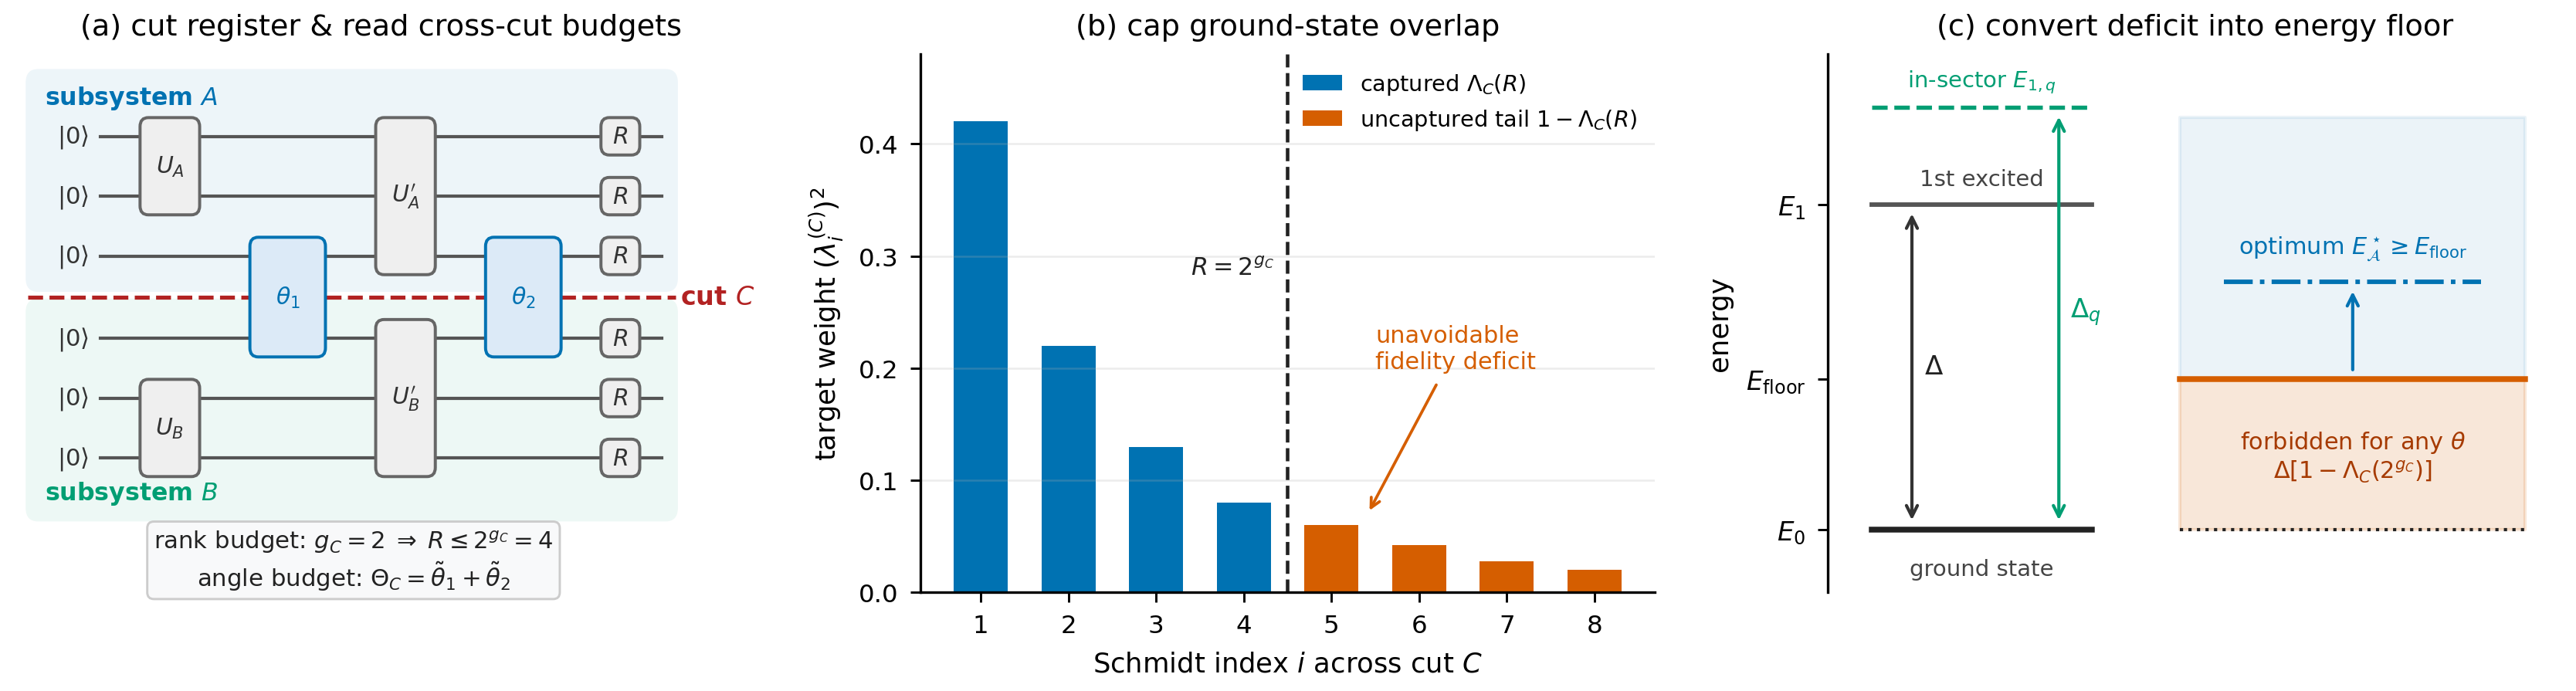
\includegraphics[width=\textwidth]{figures/schematic.png}
  \caption{Overview of the idea. \emph{(a)} A cut $C$ divides the register into
  $A$ and $B$. Only gates crossing the cut can increase the Schmidt rank across
  it: $g_C$ crossing CNOT or CZ gates allow rank at most $R=2^{g_C}$, while for
  partial entanglers the sum $\Theta_C$ of reduced gate angles $\tilde\theta_j$
  (\Cref{sec:angle}) provides an additional constraint. Cut-local gates $U_A$,
  $U_B$, and local rotations change neither budget. \emph{(b)} The resulting circuit capacity
  is compared with the Schmidt spectrum of the target ground state; any target
  weight beyond the $R$ largest components cannot be represented and gives a
  fidelity deficit $1-\Lambda_C(R)$. \emph{(c)} The spectral gap
  $\Delta=E_1-E_0$ converts this deficit into a lower bound $E_{\mathrm{floor}}$ on the energy
  error for every parameter choice. If the circuit
  preserves a symmetry, the relevant gap can instead be the larger gap
  $\Delta_q$ within that symmetry sector (\Cref{sec:sector}).}
  \label{fig:schematic}
\end{figure*}

We study when the rank certificate is informative, how much it can improve when
all cut constraints are imposed jointly, whether partial entangling angles
provide stronger information, how symmetry changes the bound, and whether the
certificate can guide the placement of entangling gates.

We derive a closed-form energy floor from the number of entangling gates
crossing each cut (\Cref{fig:schematic}). For a product-initialized circuit with
CNOT/CZ-type cross-cut entanglers that can at most double Schmidt rank, the
result is
\begin{equation*}
  E_{\calA}^{\star}-E_0\ \ge\
  \max_C\Delta\bigl[1-\Lambda_C\bigl(2^{g_C}\bigr)\bigr],
\end{equation*}
where $E_{\calA}^{\star}$ is the lowest energy achievable by the fixed circuit
architecture $\calA$. We characterize exactly when this rank-based certificate is
nonzero and when it becomes too small to resolve a chosen energy scale. We also
study the constraints from all cuts jointly and show that, within the
gap-and-fidelity framework used here, the single-cut certificate is
already within a controlled factor of the strongest floor implied by the full set
of per-cut rank constraints.

Gate count alone ignores how strongly a gate entangles. A very small $ZZ$
rotation and a maximally entangling $ZZ$ rotation receive the same rank credit
across a cut, even though their physical effects are very different. We
therefore introduce an angle-dependent certificate that uses the actual
entangling angles. The resulting bound applies to multiple entanglers crossing
the same cut and remains informative in regimes where the rank certificate has
already become negligible. We also obtain a continuous-time version that gives
a lower bound on the interaction needed to reach a desired fidelity.

We also consider symmetry. If both the initial state and every gate remain
inside one symmetry sector of the Hamiltonian, states in other sectors are
inaccessible. The relevant energy scale is then the gap within that sector rather
than the global gap. This can strengthen the certificate when the
global gap is small because of a low-energy state in another symmetry sector.

We test what these certificates do and do not tell us about circuit design. We
solve the one-dimensional problem of allocating a fixed number of entangling
gates so as to minimize the rank-based floor. The resulting allocation is
optimal for that certificate, but it does not consistently produce better
trained VQE energies in the systems we study. The same failure persists in a
disordered Heisenberg control where the certified floors lie much closer to the
trained errors. The rank certificate therefore gives a necessary condition: it can show that a circuit has insufficient
cross-cut capacity, but a small floor does not imply that the circuit is
expressive enough or easy to train.

We evaluate the certificates on the transverse-field Ising model (TFIM),
$H=-J\sum_{\langle ij\rangle}Z_iZ_j-h\sum_iX_i$, where $X,Y,Z$ are the Pauli
matrices, $\langle ij\rangle$ runs over nearest-neighbor pairs, $J$ is the
nearest-neighbor coupling, and $h$ is the transverse field (critical at $h=J$);
on the spin-$\tfrac12$ XXZ chain; on a disordered Heisenberg ensemble; and on a
Fermi--Hubbard model. For the TFIM we also use its exact free-fermion
representation to study systems up to $n=128$ qubits without many-body
truncation. These examples distinguish limits imposed by the circuit architecture from
effects that still depend on optimization.

\section{Related work}
\label{sec:related}

This work connects two questions about variational quantum circuits: how
expressive a circuit is and how difficult it is to train.

Early measures of circuit expressibility ask how broadly a parameterized circuit
can explore Hilbert space. Sim \emph{et al.}~\cite{sim2019expressibility} compare
the distribution of states generated by a circuit with the Haar distribution and
also study its average entangling capability. Nakaji and
Yamamoto~\cite{nakaji2021expressibility} analyze the approximation power of
alternating layered ans\"atze using a Hilbert--Schmidt distance, while Haug
\emph{et al.}~\cite{haug2021capacity} relate the effective dimension and geometry
of a parameterized circuit to its number of two-qubit gates. These approaches compare circuit families in general, but they are not tied to a
particular target ground state. A circuit can score well under a global
expressibility measure and still lack the specific entanglement structure
required by one Hamiltonian. We instead consider a target-specific question: for a fixed Hamiltonian and
circuit architecture, can the architecture be shown to have an unavoidable
energy error?

Trainability studies address the other major source of VQE failure. McClean
\emph{et al.}~\cite{mcclean2018barren} showed that gradients can become
exponentially small in parameterized quantum circuits, producing barren plateaus.
Later work showed that this behavior depends on the cost function and circuit
structure~\cite{cerezo2021cost} and can also be induced by
noise~\cite{wang2021noiseinduced}. Holmes \emph{et al.}~\cite{holmes2022connecting}
further connected high expressibility with small gradients, showing that making a
circuit more expressive can itself make optimization harder. These results
explain why an architecture that \emph{can} represent a good state may still be
difficult to train. They do not, however, determine whether such a good state
exists inside the circuit family in the first place. Our bounds address whether a good state exists within the circuit family and do
not depend on gradients, initialization, or the
optimizer. When the resulting floor is very small compared with the trained error, the
certificate alone does not identify the source of the remaining error; it may
arise from optimization or from structural restrictions not captured by the
bound.

Our use of Schmidt rank is closely connected to tensor-network descriptions of
many-body states. Vidal showed that one-dimensional states with bounded Schmidt
rank can be represented and simulated efficiently~\cite{vidal2003efficient,vidal2004efficient},
forming the basis for matrix-product-state (MPS) methods and the density-matrix
renormalization group~\cite{schollwock2011density}. Instead of asking
whether a low-rank state is easy to represent classically, we ask whether a
shallow quantum circuit has enough cross-cut capacity to produce a target state
with a given Schmidt spectrum. The relevant circuit fact is that a two-qubit
gate can increase the state Schmidt rank across a bipartition only by a bounded
factor~\cite{nielsen2003quantum,vatan2004optimal,balakrishnan2010operator}. These results provide the rank constraint used here, but by
themselves they do not give an energy penalty for failing to reproduce the target
Schmidt spectrum. We obtain that penalty by combining the circuit rank limit with
the target-specific Schmidt coefficients and the spectral gap of the
Hamiltonian.

The behavior of the target Schmidt spectrum is also well understood in many
one-dimensional systems. Gapped ground states satisfy entanglement area
laws~\cite{eisert2010colloquium}, while critical systems can show logarithmic
growth of entanglement with system
size~\cite{calabrese2004entanglement,laflorencie2016quantum,sachdev2011quantum}.
The relation between spectral gap and entanglement is not
one-to-one~\cite{gottesman2010entanglement}. In our certificate, the Schmidt-spectrum tail controls the fidelity deficit,
while the spectral gap converts that deficit into an energy floor. A target can
therefore become harder to approximate in fidelity while its certified energy
penalty remains small because the gap is closing. The large-system Ising results
in \Cref{sec:scaling} show this behavior explicitly.

A second line of work asks how quickly gates or interactions can create
entanglement. Entangling power characterizes the ability of two-qubit gates to
generate entanglement~\cite{kraus2001optimal,nielsen2003quantum}, while
entangling-rate bounds constrain how quickly entanglement can grow under
continuous Hamiltonian evolution~\cite{bravyi2007upper,vanacoleyen2013entanglement}.
Quantum speed limits similarly bound how far a state can move in Hilbert space
during a finite evolution~\cite{mandelstam1945uncertainty}, and recent work has
related two-qubit entanglement growth to quantum Fisher
information~\cite{saleem2026speed}. This motivates retaining the gate angle in addition to its rank contribution. Rank counting treats an arbitrarily weak
entangler, as soon as it is nonzero, in the same way as a strong entangler. We
instead bound how far each partial entangler can move the state away from a
low-Schmidt-rank set and add these changes across the circuit. This gives the
angle-budget certificate and its continuous-time pulse-area version.

Other work focuses on constructing or adapting variational circuits rather than
certifying a fixed architecture. The adaptive derivative-assembled pseudo-Trotter
VQE (ADAPT-VQE) grows an ansatz iteratively by selecting operators during the
optimization~\cite{grimsley2019adaptive}. Other approaches choose orbital
orderings or qubit permutations to place strongly correlated degrees of freedom
near one another~\cite{tubman2018postponing,tkachenko2021permvqe}. Joch
\emph{et al.}~\cite{joch2025entanglement} use entanglement information directly
when constructing variational circuits, while Green
\emph{et al.}~\cite{green2025schmidt} optimize state preparation using
Schmidt-spectrum information. These methods construct or adapt circuit architectures. We instead consider a
fixed architecture and bound what it can achieve before training. We also test the certificate as a rule for allocating entangling gates. In our experiments, exact minimization of the certificate does not consistently
produce the lowest trained energy.

Recent architecture-search work also separates structural capacity from
optimization performance. HamQASBench~\cite{niu2026hamqasbench} evaluates
quantum architecture-search methods using Hamiltonian properties such as
entanglement, degeneracy, and connectivity, with the goal of separating
structural limitations from failures of the search procedure. L\"osl
\emph{et al.}~\cite{losl2026variational} study circuits with sparse long-range
entangling gates and show that enlarging the accessible operator space does not
by itself guarantee good trainability. Alavi \emph{et al.}~\cite{alavi2026gram}
study certified resource continuation, in which richer representations are
warm-started from cheaper ones, and show that such continuation cannot overcome
a Schmidt-rank ceiling imposed by the final representation; that ceiling is
closely related to the rank constraint used here. For a fixed architecture, we instead derive a
lower bound on its achievable energy that is independent of how the circuit is
trained.

There are also more direct bounds on circuit or ground-state energy. In modular
VQE, Khait \emph{et al.}~\cite{khait2023distributed} use the limited number of
operations between modules to constrain the bipartite entanglement that can be
generated across a module boundary. This provides a related cross-cut entanglement constraint. We compare that
capacity with the Schmidt spectrum of a specific target state and convert the
resulting fidelity deficit into an energy floor. Mishra \emph{et al.}~\cite{mishra2024classically} instead
derive lower bounds on the energy achievable by a specified circuit in the
presence of depolarizing noise, using Lagrangian duality and a
matrix-product-operator approximation. Their bound concerns noise-induced
limitations, whereas ours concerns the noiseless representational limitation of
the circuit itself. Dual variational quantum eigensolver (dual-VQE)
methods~\cite{westerheim2024dual} address yet another quantity: they lower-bound
the true ground-state energy $E_0$. Our certificate does not lower-bound $E_0$;
it lower-bounds the best energy $E_{\calA}^{\star}$ attainable by a particular
circuit architecture.

Existing work addresses generic expressibility, optimization difficulty,
entanglement generation, circuit construction, and related energy bounds. We seek a target-specific lower bound on the achievable energy of a fixed,
noiseless circuit from its entanglement capacity.

We combine cut-wise gate-count limits with the target Schmidt spectrum and
spectral gap, then extend the construction to joint cut constraints, gate
angles, pulse areas, and symmetry sectors.

\section{Rank-based energy certificate}
\label{sec:rank}

Consider a cut $C$ that
divides the $n$-qubit register into two groups $A$ and $B$, with $|A|$ and
$|B|=n-|A|$ qubits; a chain of $n$ qubits has $n-1$ contiguous cuts. Across this
cut, any normalized pure state can be written in Schmidt form,
\begin{equation}
  \label{eq:schmidt}
  \ket{\psi}=\sum_{i=1}^{d_C}\lambda_i^{(C)}\ket{a_i}\ket{b_i},
\end{equation}
where $\{\ket{a_i}\}$ and $\{\ket{b_i}\}$ are orthonormal states of $A$ and $B$,
the coefficients are ordered as $\lambda_1^{(C)}\ge\lambda_2^{(C)}\ge\cdots>0$,
and $\sum_i(\lambda_i^{(C)})^2=1$. The squared coefficients give the weight of
each Schmidt component, while $d_C$ is the Schmidt rank across the cut. We write
$\rank_C(\psi):=d_C$ for the Schmidt rank of $\ket{\psi}$ across $C$; it can
never exceed $2^{\min(|A|,|B|)}$, the dimension of the smaller side.

Let $\ket{\psi_0}$ be the target ground state. If a circuit can
produce states of Schmidt rank at most $R$ across $C$, the best possible squared
overlap with $\ket{\psi_0}$ is obtained by keeping its $R$ largest Schmidt
components~\cite{eckart1936approximation} (\Cref{app:fidelity}). We therefore
define:

\begin{definition}[Fidelity capacity]
\label{def:lambda}
For the target ground state $\ket{\psi_0}$ with Schmidt coefficients
$\lambda_i^{(C)}$ across cut $C$,
\begin{equation}
  \label{eq:lambda}
  \Lambda_C(R):=\sum_{i=1}^{\min(R,d_C)}\bigl(\lambda_i^{(C)}\bigr)^2 .
\end{equation}
\end{definition}

$\Lambda_C(R)$ is the largest fraction of the target state that a
Schmidt-rank-$R$ state can capture across cut $C$. It increases with $R$ and
reaches $1$ once $R\ge d_C$.

A circuit starting from a product state has Schmidt rank one across every cut.
Gates acting entirely inside $A$ or $B$ do not change that rank. The class considered here includes CNOT, CZ, and $ZZ$ rotations
$e^{-i\theta Z\otimes Z}$, each of which can at most double the Schmidt rank
across the cut (\Cref{app:rank}). Therefore, after $g_C$ such gates cross $C$, every state produced
by the circuit has Schmidt rank at most $2^{g_C}$. Its squared overlap with the
ground state, $f$, is consequently bounded by
\begin{equation}
  f\ \le\ \Lambda_C\bigl(2^{g_C}\bigr).
\end{equation}

The spectral gap converts this fidelity limitation into an energy limitation. Let
$E_0$ and $E_1$ be the two lowest energies of $H$, with a nondegenerate ground
state, and let $\Delta=E_1-E_0$. If a state has squared ground-state overlap $f$,
the remaining probability $1-f$ lies in excited states with energy at least
$E_1$. Its energy $E$ therefore satisfies
\begin{equation}
  E-E_0\ \ge\ \Delta(1-f).
\end{equation}
Combining the two observations, and maximizing over cuts, gives the rank-based
certificate (proof in \Cref{app:rank}).

\begin{theorem}[Rank-budget certificate]
\label{thm:main}
Let $\calA$ be a product-initialized circuit architecture whose cross-cut
entanglers each at most double the Schmidt rank across any cut (\Cref{app:rank}),
with $g_C$ of them crossing cut $C$, and let
$\Estar:=\min_\theta\bra{\psi_\calA(\theta)}H\ket{\psi_\calA(\theta)}$ be the
lowest energy it can reach over all parameters $\theta$. Then
\begin{equation}
  \label{eq:multi}
  \boxed{\;
  \Estar - E_0 \ \ge\ \calC_{\calA}(H)
  :=\max_C\,\Delta\bigl[1-\Lambda_C(2^{g_C})\bigr].
  \;}
\end{equation}
\end{theorem}

The cut that gives the largest floor is the \emph{bottleneck} cut: it is where
the circuit has the least entanglement capacity relative to what the target
requires. The numerical circuits used later are described in
\Cref{app:numerics}.

The theorem also applies to arbitrary bipartitions, provided $g_C$ counts every
gate crossing the cut. We use contiguous cuts for most one-dimensional examples
and general bipartitions in the Fermi--Hubbard example (\Cref{sec:hubbard}).

The certificate is one-sided. A positive floor can rule out a requested
accuracy, but a small or zero floor does not imply that the architecture will
succeed. Other restrictions, including gate
ordering and optimization difficulty, can still prevent the circuit from reaching
the ground state.

All numerical certificate values in this work use full finite-dimensional
diagonalization or the free-fermion representation of the Ising model without
many-body truncation. They
are evaluated in standard floating-point arithmetic rather than with
interval-certified numerics; details are given in \Cref{app:numerics}.

\subsection{Informative window and triviality threshold}
\label{sec:window}

The rank certificate has a built-in limitation: after enough crossing gates have
been added, rank alone can no longer distinguish the circuit from the target.
Two thresholds are relevant. The exact threshold occurs when the circuit can
support the full Schmidt rank of the target, $2^{g_C}\ge d_C$, at which point
the rank-based floor at that cut is zero; because $d_C\le2^{\min(|A|,|B|)}$,
this always happens once $g_C\ge\min(|A|,|B|)$ by dimension counting alone. For
a chosen energy tolerance, an earlier effective threshold occurs when the floor
becomes small on the energy scale of interest. To quantify this, let
\begin{equation}
  \label{eq:Reps}
  R_C(\varepsilon):=\min\{R:\ 1-\Lambda_C(R)\le\varepsilon\}
\end{equation}
be the number of Schmidt components needed to capture all but a fraction
$\varepsilon$ of the target weight. Once
\begin{equation}
  g_C\ \ge\ g_C^\star(\varepsilon):=\bigl\lceil\log_2 R_C(\varepsilon)\bigr\rceil ,
\end{equation}
the floor at $C$ is at most $\Delta\varepsilon$ (\Cref{prop:window} in
\Cref{app:rank}). The threshold $g_C^\star(\varepsilon)$ depends on the tail of the
Schmidt spectrum, not on the entanglement entropy alone.

\begin{figure*}[t]
  \centering
  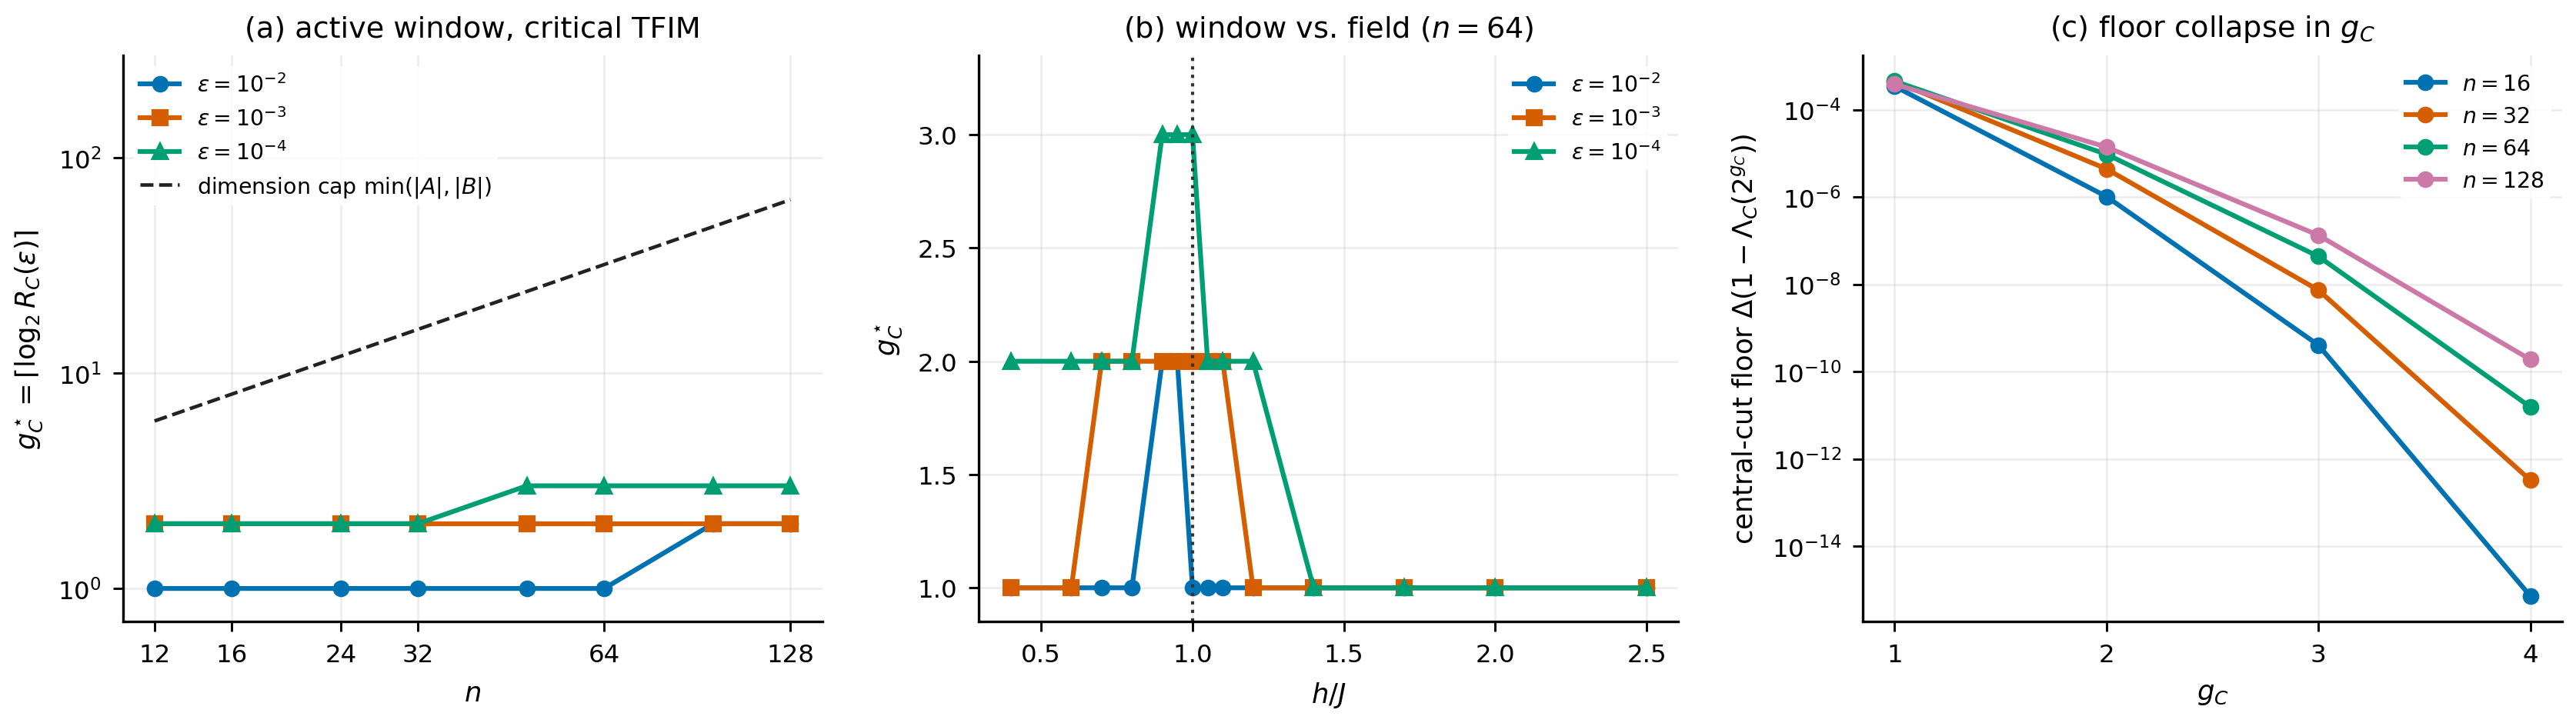
\includegraphics[width=\textwidth]{figures/window.png}
  \caption{Informative window of the rank certificate on the critical open TFIM,
  computed from exact free-fermion Schmidt spectra.
  \emph{(a)} Triviality threshold
  $g_C^\star(\varepsilon)=\lceil\log_2 R_C(\varepsilon)\rceil$ at the central
  cut versus $n$, compared with the dimension cap $\min(|A|,|B|)$. The threshold
  grows slowly, approximately logarithmically over the sizes shown, while the
  dimension cap grows linearly.
  \emph{(b)} Threshold versus transverse field $h/J$ at $n=64$ (dotted line:
  $h/J=1$).
  \emph{(c)} Central-cut floor versus $g_C$, dropping by roughly two orders of
  magnitude per added gate.}
  \label{fig:window}
\end{figure*}

\Cref{fig:window} maps this window for the critical open TFIM using exact
free-fermion spectra (\Cref{sec:scaling}). Even up to $n=128$, the threshold
$g_C^\star(\varepsilon)$ reaches only $2$--$3$ gates across the central cut,
while the dimension cap $\min(|A|,|B|)$ grows linearly, and each additional
crossing gate suppresses the certified floor by roughly two orders of magnitude.
For these critical one-dimensional chains, the certificate is therefore informative only for roughly $g_C\lesssim3$. This narrow window contributes to the large floor--error separation seen later
in the TFIM allocation experiment (\Cref{sec:allocation}).

\section{The angle-budget certificate}
\label{sec:angle}

Rank counts whether a cross-cut gate can increase Schmidt rank, but it ignores
how strongly the gate acts. For example, $e^{-i10^{-3}Z\otimes Z}$ and
$e^{-i(\pi/4)Z\otimes Z}$ receive the same rank credit, even though the first
gate is very close to the identity. We therefore retain the amount of entangling
rotation applied across each cut.

We consider cross-cut gates of the form $e^{-i\theta P\otimes Q}$, where $P$ acts
on $A$, $Q$ acts on $B$, and both are Hermitian operators that square to the
identity (for example, Pauli strings). The entangling content of such a gate is
measured by its reduced angle
\begin{equation}
  \label{eq:cost}
  \tilde\theta:=\min_{k\in\mathbb{Z}}\bigl|\theta-k\pi/2\bigr|\ \in[0,\pi/4].
\end{equation}
The periodic definition is needed because at multiples of $\pi/2$ the gate again
factors across the cut, being proportional to $I\otimes I$ or to $P\otimes Q$.
Thus $\tilde\theta=0$ whenever the gate factors into operations on the two sides
of the cut, and $\tilde\theta$ reaches
its maximum $\pi/4$ halfway between two such points, as for CNOT and CZ, which
are equivalent to $e^{-i(\pi/4)Z\otimes Z}$ up to cut-local gates.

One such gate can move the state away from the set of Schmidt-rank-$K$ states
by at most $\tilde\theta$, while cut-local gates do not move it at all. The corresponding distance increases additively across successive cross-cut
gates. The distance
is measured by the Fubini--Study angle $\arccos|\braket{\psi}{\phi}|$ between
normalized states; the precise statement and proof are given in
\Cref{lem:distance} of \Cref{app:angle}.

If every crossing gate is counted by angle, with total angle budget
\begin{equation}
  \Theta_C:=\sum_j\tilde\theta_j
\end{equation}
across $C$ and angular distance $\alpha_C:=\arccos\sqrt{\Lambda_C(1)}$ between
the target and the nearest product state across $C$, the bound becomes
\begin{equation}
  \label{eq:speedfloor}
  E-E_0\ \ge\ \Delta\,\sin^2\bigl([\alpha_C-\Theta_C]_+\bigr),
\end{equation}
where $[x]_+:=\max\{x,0\}$. The target lies a distance $\alpha_C$ from the
nearest product state. Cross-cut
interactions can close that distance only at a rate limited by their total
entangling angle. If the available angle $\Theta_C$ is too small, some distance
from the target necessarily remains, which produces a nonzero energy floor.

The hybrid theorem allows each gate to contribute through either its rank or its
angle (\Cref{thm:angle} in \Cref{app:angle}). The choice $J=\varnothing$
reproduces the rank certificate of \Cref{thm:main}. Choosing all gates in $J$
gives the all-angle member of the hybrid bound; \eqref{eq:speedfloor} follows
separately from the distance to the product-state set and coincides with that
member when $\Lambda_C(2^g)=1$, i.e., when the allowed rank already captures the
full target Schmidt support. The hybrid bound is never weaker than the
corresponding Hilbert-space triangle bound and can be strictly stronger. It
is tight for one crossing gate and for rank-two targets with $\Theta_C\le\pi/4$
under arbitrary cut-local operations (\Cref{app:tight}), is numerically
saturated in the controlled rank-two tests studied here, and extends to
arbitrary two-qubit gates through their canonical decomposition.

The angle bound also extends to continuous-time control. Suppose the circuit is
replaced by a time-dependent control Hamiltonian
\begin{equation}
  H_{\mathrm{ctrl}}(t)=H_A(t)+H_B(t)+\sum_kJ_k(t)\,P_k\otimes Q_k ,
\end{equation}
where $H_A(t)$ and $H_B(t)$ act within $A$ and $B$, and the couplings $J_k(t)$
multiply cross-cut terms of the form above. The total cross-cut interaction over
a duration $T$ is measured by the pulse area
$\Theta_C(T):=\sum_k\int_0^T|J_k(t)|\,dt$. To reach squared fidelity $F$ with the
target, this area must satisfy $\Theta_C(T)\ge[\alpha_C-\arccos\sqrt{F}]_+$
(\Cref{cor:pulse}). In particular, for a single cross-cut coupling bounded by
$|J(t)|\le J_{\max}$, as in pulse-level VQE~\cite{meitei2021gatefree}, one has
$\Theta_C(T)\le J_{\max}T$, so
\begin{equation}
  \label{eq:pulsetime}
  T\ \ge\ \frac{[\alpha_C-\arccos\sqrt{F}]_+}{J_{\max}},
\end{equation}
with $J_{\max}$ replaced by $\sum_kJ_{k,\max}$ when several couplings
$|J_k(t)|\le J_{k,\max}$ cross $C$ simultaneously. Bounded coupling strength therefore implies a minimum interaction time needed
to create the target's cross-cut entanglement.
For the critical open TFIM, $\alpha_C$ at the
central cut grows from $0.344$ at $n=8$ to $0.498$ at $n=128$, so reaching
$F=0.99$ requires a pulse area of at least $0.24$ at $n=8$ and $0.40$ at
$n=128$.

The angle certificate is a pre-training bound when the entangling angles are
fixed or constrained by hardware; in the constrained case it is evaluated using the
largest allowed reduced-angle budget. If those angles are themselves freely optimized without
any bound, the final angles are not known before training, so the result should
instead be interpreted as a post-training diagnostic.

\subsection{Numerical validation of the angle budget}

We use a four-qubit example for which the angle bound can be saturated,
\begin{equation}
  \label{eq:Htest}
  H_{\mathrm{test}}=X_1X_2+Y_1Y_2+Z_1Z_2-3\,(Z_0+Z_3).
\end{equation}
Its ground state contains a singlet across the central cut, with the outer qubits
pinned by strong fields ($E_0=-9$, $\Delta=4$), and therefore has Schmidt rank two
there, with $\Lambda_C(1)=0.5$ and $\Lambda_C(2)=1$. This rank-two target
provides a controlled test of tightness. The circuit places $p\in\{1,2,3\}$ gates
$e^{-i\theta Z_1Z_2}$ at fixed $\theta$ on the central bond, with independent
single-qubit rotations $R_y$ and $R_z$ on all qubits before, between, and after
them, where $R_\alpha(\theta)=e^{-i\theta\sigma_\alpha/2}$ for
$\sigma_\alpha\in\{X,Y,Z\}$. All rotations are trained from $20$ random
restarts.

\begin{table}[t]
\centering
\caption{Angle-budget certificate on the four-qubit singlet target ($E_0=-9$,
$\Delta=4$, $\Lambda_C(1)=0.5$, $\Lambda_C(2)=1$), with $p$ gates
$e^{-i\theta ZZ}$ at fixed $\theta$ across the central cut and all single-qubit
gates trained ($20$ restarts); ``angle floor'' is \Cref{thm:angle}. The rank
floor is ${\sim}10^{-15}$ throughout.}
\label{tab:angle}
{\small\setlength{\tabcolsep}{5pt}
\begin{tabular}{ccccc}
\toprule
$p$ & $\theta$ & $E_{\mathrm{VQE}}-E_0$ & angle floor & triangle floor\\
\midrule
1 & $0.05$ & $1.8003$ & $1.8003$ & $1.7073$\\
1 & $0.10$ & $1.6027$ & $1.6027$ & $1.3954$\\
1 & $0.15$ & $1.4090$ & $1.4090$ & $1.0653$\\
1 & $0.25$ & $1.0411$ & $1.0411$ & $0.3556$\\
2 & $0.05$ & $1.6027$ & $1.6027$ & $1.3946$\\
2 & $0.10$ & $1.2212$ & $1.2212$ & $0.7110$\\
2 & $0.15$ & $0.8707$ & $0.8707$ & $0$\\
2 & $0.25$ & $0.3171$ & $0.3171$ & $0$\\
3 & $0.05$ & $1.4090$ & $1.4090$ & $1.0619$\\
3 & $0.10$ & $0.8707$ & $0.8707$ & $0$\\
3 & $0.15$ & $0.4333$ & $0.4333$ & $0$\\
3 & $0.25$ & $0.0050$ & $0.0050$ & $0$\\
\bottomrule
\end{tabular}}
\end{table}

The trained values agree with the angle bound of \Cref{thm:angle} to four
decimal places in all $12$ settings (\Cref{tab:angle} and \Cref{fig:angle}a),
including the eight with two or three gates per cut, where the Hilbert-space
triangle bound is weaker and is zero in five cases. The rank certificate, in contrast, is
already zero, because one nontrivial crossing gate is enough to allow the full
Schmidt rank of the target. Finitely many restarts cannot prove that the optimum
equals the bound, so we describe this as numerical saturation.

We next evaluate the angle certificate on the critical open TFIM at $n=8$
($E_0=-9.8380$, $\Delta=0.3691$), using $p$ layers that each apply $R_yR_z$ to
every qubit and then $e^{-i\theta ZZ}$ on every bond at a common fixed $\theta$,
followed by a final rotation layer; only the rotations are trained ($10$
restarts). Gates on other bonds do not cross a given cut, so \Cref{thm:angle}
applies at each cut with $p$ gates of cost $\theta$, and we report the largest
floor over cuts (\Cref{tab:angle_tfim} and \Cref{fig:angle}b).

\begin{table}[t]
\centering
\caption{Critical TFIM, $n=8$ (open, $E_0=-9.8380$, $\Delta=0.3691$), $p$
layers of $e^{-i\theta ZZ}$ on every bond at fixed $\theta$, rotations trained
($10$ restarts); ``angle'', ``triangle'', and ``rank'' are the angle-budget floor of
\Cref{thm:angle}, the triangle floor, and the rank floor, each maximized over
cuts.}
\label{tab:angle_tfim}
{\small\setlength{\tabcolsep}{4pt}
\begin{tabular}{cccccc}
\toprule
$p$ & $\theta$ & $E_{\mathrm{VQE}}-E_0$ & angle & triangle & rank\\
\midrule
1 & $0.02$ & $0.358$ & $3.7{\times}10^{-2}$ & $2.8{\times}10^{-2}$ & $1.7{\times}10^{-4}$\\
1 & $0.10$ & $0.213$ & $2.2{\times}10^{-2}$ & $1.7{\times}10^{-4}$ & $1.7{\times}10^{-4}$\\
2 & $0.02$ & $0.299$ & $3.3{\times}10^{-2}$ & $1.4{\times}10^{-2}$ & $5.6{\times}10^{-8}$\\
2 & $0.10$ & $0.163$ & $7.6{\times}10^{-3}$ & $5.6{\times}10^{-8}$ & $5.6{\times}10^{-8}$\\
3 & $0.02$ & $0.257$ & $2.9{\times}10^{-2}$ & $9.7{\times}10^{-13}$ & $9.7{\times}10^{-13}$\\
3 & $0.05$ & $0.175$ & $1.4{\times}10^{-2}$ & $9.7{\times}10^{-13}$ & $9.7{\times}10^{-13}$\\
4 & $0.02$ & $0.230$ & $2.5{\times}10^{-2}$ & ${\sim}0$ & ${\sim}0$\\
4 & $0.05$ & $0.154$ & $7.6{\times}10^{-3}$ & ${\sim}0$ & ${\sim}0$\\
\bottomrule
\end{tabular}}
\end{table}

\begin{figure}[tb]
  \centering
  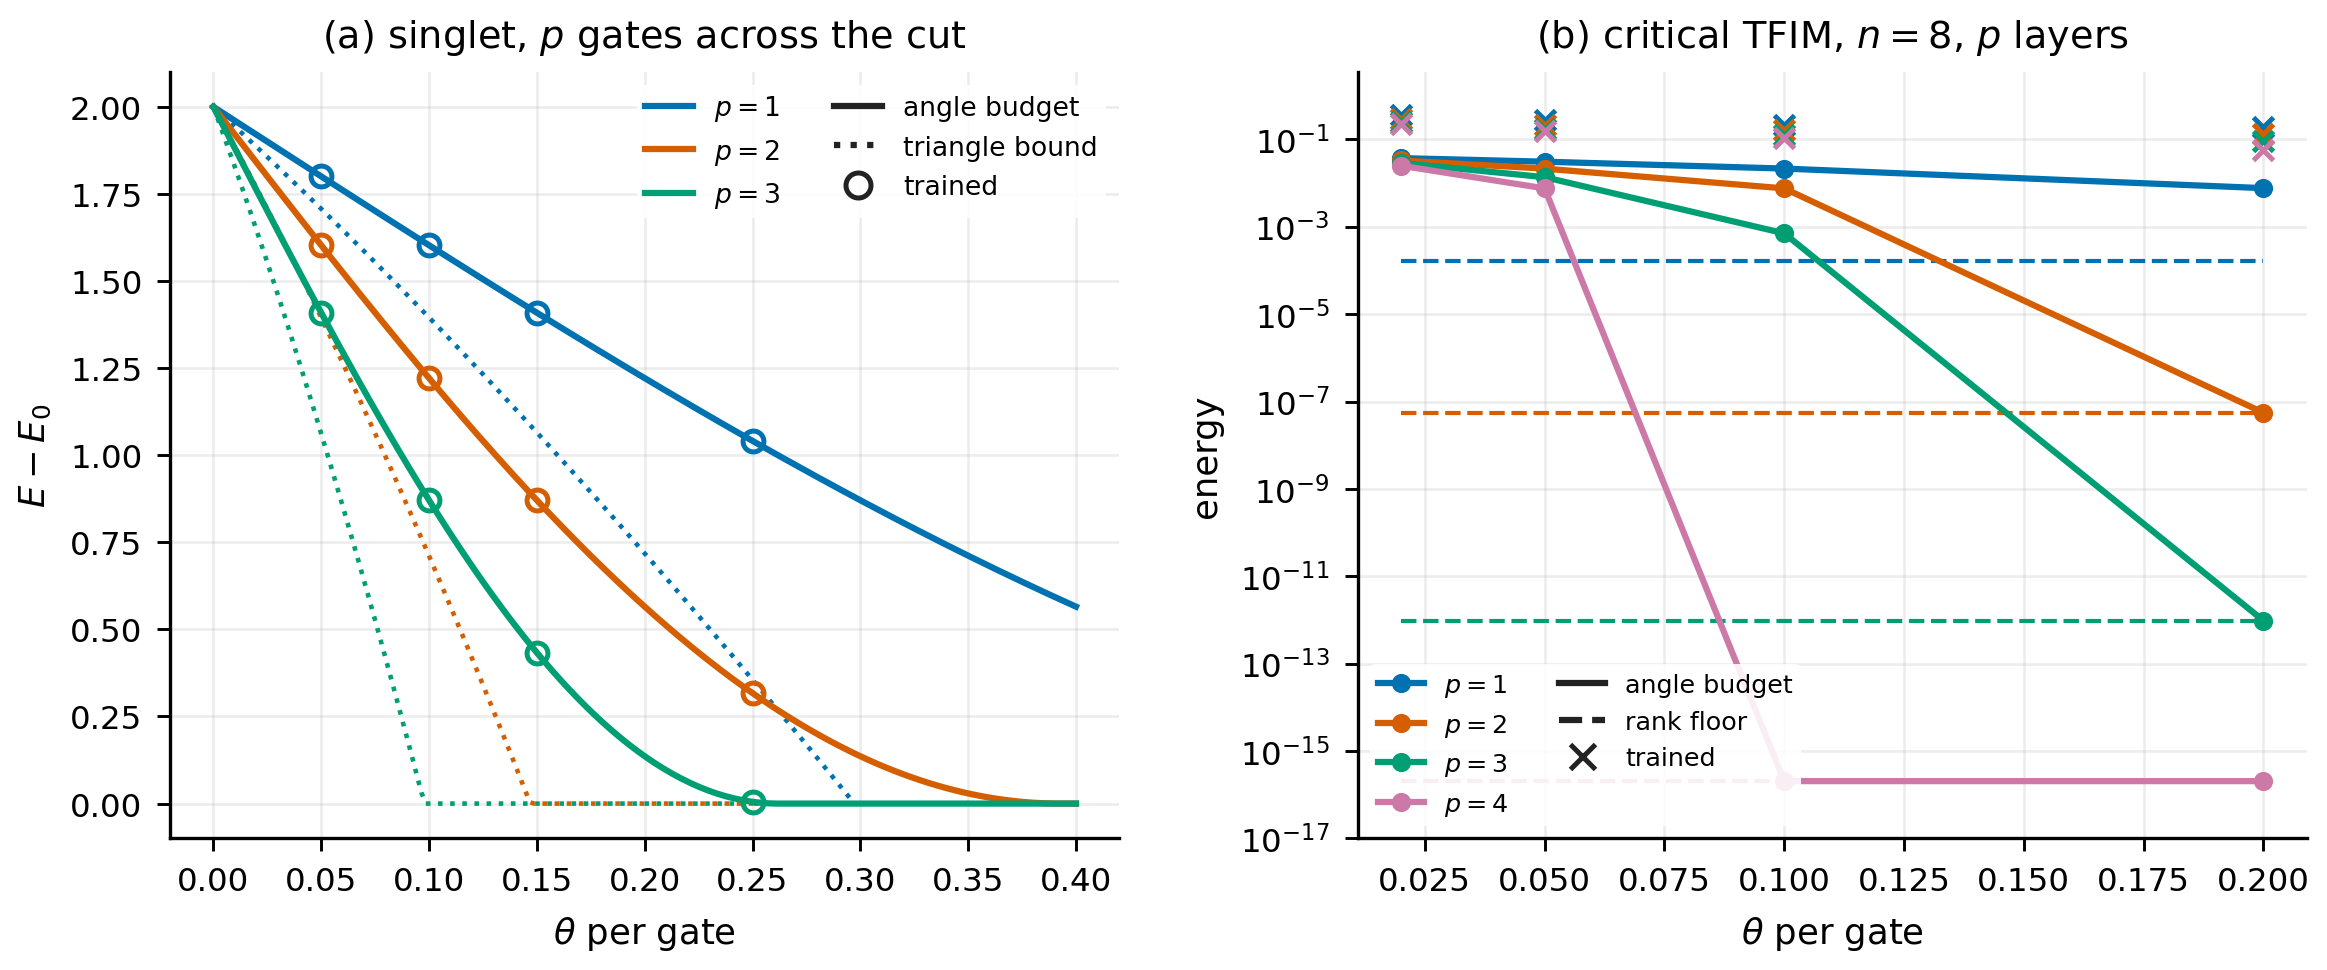
\includegraphics[width=\columnwidth]{figures/angle.png}
  \caption{Angle-budget certificate. \emph{(a)} Four-qubit singlet target with
  $p$ gates of angle $\theta$ across the central cut: trained VQE errors
  (circles) lie on \Cref{thm:angle} (solid) for $p=1,2,3$, whereas the triangle
  bound (dotted) is weaker and the rank floor vanishes. \emph{(b)} Critical open
  TFIM, $n=8$: angle-budget floor (solid), rank floor (dashed, collapsing with
  $p$), and trained errors (crosses) for $p=1$--$4$ layers.}
  \label{fig:angle}
\end{figure}

The rank floor becomes negligible after only a few layers, because every nonzero
$ZZ$ gate receives a full rank credit: it falls from $1.7\times10^{-4}$ at $p=1$
to below $10^{-12}$ at $p=3$. The angle floor remains nonzero in the same regime. For weak gates ($\theta=0.02$) it continues to give floors of
$2.5$--$3.7\times10^{-2}$ for every $p\le4$, within roughly one order of
magnitude of the trained error (at most a factor of $9.6$). As $p\theta$ grows
toward the angles the target actually requires, the angle floor decreases and
eventually meets the rank floor.

\section{The symmetry-sector certificate}
\label{sec:sector}

Suppose the global first excited state lies outside the symmetry sector of the
circuit. If the circuit is restricted to another symmetry sector, that
excitation is inaccessible and should not set the relevant energy scale; using
the global gap then gives an unnecessarily weak certificate.

A symmetry sector is the subspace of states with a fixed eigenvalue $q$ of a
conserved operator $Q$, where $[H,Q]=0$. If the initial state and every gate
remain in one sector $q$, the entire variational circuit remains in that sector.
The lowest accessible excitation is therefore not necessarily the first excited
state of the full Hamiltonian; it is the first excited state inside sector $q$.
Writing $E_{0,q}$ and $E_{1,q}$ for the two lowest energies within the sector, we
denote the corresponding gap by
\begin{equation}
  \Delta_q:=E_{1,q}-E_{0,q}.
\end{equation}
The same rank argument then applies with $\Delta_q$ in place of the global gap
$\Delta$. If the lowest state in the sector is nondegenerate and has fidelity
capacity $\Lambda_{C,q}$, every state prepared by the circuit obeys
\begin{equation}
  \label{eq:sectorfloor}
  E - E_{0,q}\ \ge\ \Delta_q\bigl[1-\Lambda_{C,q}(2^{g_C})\bigr]
\end{equation}
across every cut $C$ (\Cref{thm:sector}, stated with full hypotheses and proved
in \Cref{app:sector}). When the global ground state lies in sector $q$, as in the
examples below, $E_{0,q}=E_0$ and $\Lambda_{C,q}=\Lambda_C$. The Schmidt part of
the certificate is unchanged; only the energy scale is replaced by the lowest
excitation that the circuit can actually access.

For the TFIM, the spin-flip parity $P=\prod_iX_i$ commutes with $H$, and at
finite $n$ the ground state lies in the $P=+1$ sector. In the ordered phase
($h<J$), the two lowest states have opposite parity and become nearly degenerate
as the system grows. This makes the global gap very small. A parity-preserving
circuit starting in the $P=+1$ sector cannot access the $P=-1$ partner, so the
relevant gap is instead the much larger spacing to the next $P=+1$ state. At
$h/J=0.5$, the ratio $\Delta_q/\Delta$ increases from $360$ at $n=6$ to
$2.94\times10^4$ at $n=12$, approximately as $e^{0.73n}$
(\Cref{tab:sectorscaling} in \Cref{app:sector}).

We compare two circuit families. The first starts from
$\ket{+}^{\otimes n}$, where $\ket{+}=(\ket0+\ket1)/\sqrt2$, and uses $R_x$
rotations with $e^{-i\theta ZZ}$ entanglers; it preserves $P=+1$ for all
parameters. The second is the standard hardware-efficient ansatz
(HEA)~\cite{kandala2017hardware}, with
$R_y$ and $R_z$ rotations and CNOT entanglers starting from $\ket{0}^{\otimes n}$;
it does not preserve parity (\Cref{app:sector}), so \eqref{eq:sectorfloor} does
not apply to it.

\begin{table}[t]
\centering
\caption{Global versus sector-resolved certificate on the periodic TFIM at
$n=8$, central cut ($g=g_C$), $P=+1$ sector. Floors are certified lower bounds on the
energy error; VQE rows report trained energy errors above $E_0$ for the
parity-preserving $R_x$+$ZZ$ circuit (covered by \eqref{eq:sectorfloor}) and for
the symmetry-breaking HEA (not covered). At $g=0$ the parity-preserving family
contains only $\ket{+}^{\otimes n}$.}
\label{tab:sector}
{\footnotesize\setlength{\tabcolsep}{2.6pt}
\begin{tabular}{lcccc}
\toprule
 & $g=0$ & $g=1$ & $g=2$ & $\Delta_q/\Delta$\\
\midrule
\multicolumn{5}{l}{\emph{Ordered} $h/J=0.5$: $\Delta=1.46{\times}10^{-3}$,
 $\Delta_q=2.284$}\\
$\Lambda_C(2^g)$    & $0.5177$ & $0.9993$ & $0.9999$ & \\
global floor       & $7.0{\times}10^{-4}$ & $1.1{\times}10^{-6}$ & $1.9{\times}10^{-7}$ & \\
sector floor       & $\mathbf{1.10}$ & $1.7{\times}10^{-3}$ & $3.0{\times}10^{-4}$ & $1569$\\
parity VQE         & $4.509$ & $2.145$ & $1.404$ & \\
HEA VQE            & $0.0091$ & $0.0022$ & $0.0022$ & \\[3pt]
\multicolumn{5}{l}{\emph{Critical} $h/J=1$: $\Delta=0.1970$, $\Delta_q=1.561$}\\
$\Lambda_C(2^g)$    & $0.7508$ & $0.9827$ & $0.9997$ & \\
global floor       & $4.9{\times}10^{-2}$ & $3.4{\times}10^{-3}$ & $5.7{\times}10^{-5}$ & \\
sector floor       & $0.389$ & $2.7{\times}10^{-2}$ & $4.5{\times}10^{-4}$ & $7.9$\\
parity VQE         & $2.252$ & $0.765$ & $0.499$ & \\
HEA VQE            & $0.252$ & $0.138$ & $0.121$ & \\[3pt]
\multicolumn{5}{l}{\emph{Paramagnetic} $h/J=2$: $\Delta=2.003$, $\Delta_q=4.569$}\\
$\Lambda_C(2^g)$    & $0.9645$ & $0.9858$ & $1.0000$ & \\
global floor       & $7.1{\times}10^{-2}$ & $2.8{\times}10^{-2}$ & $2.6{\times}10^{-5}$ & \\
sector floor       & $0.162$ & $6.5{\times}10^{-2}$ & $6.0{\times}10^{-5}$ & $2.3$\\
parity VQE         & $1.018$ & $0.187$ & $0.137$ & \\
HEA VQE            & $1.018$ & $0.145$ & $0.136$ & \\
\bottomrule
\end{tabular}}
\end{table}

\begin{figure*}[t]
  \centering
  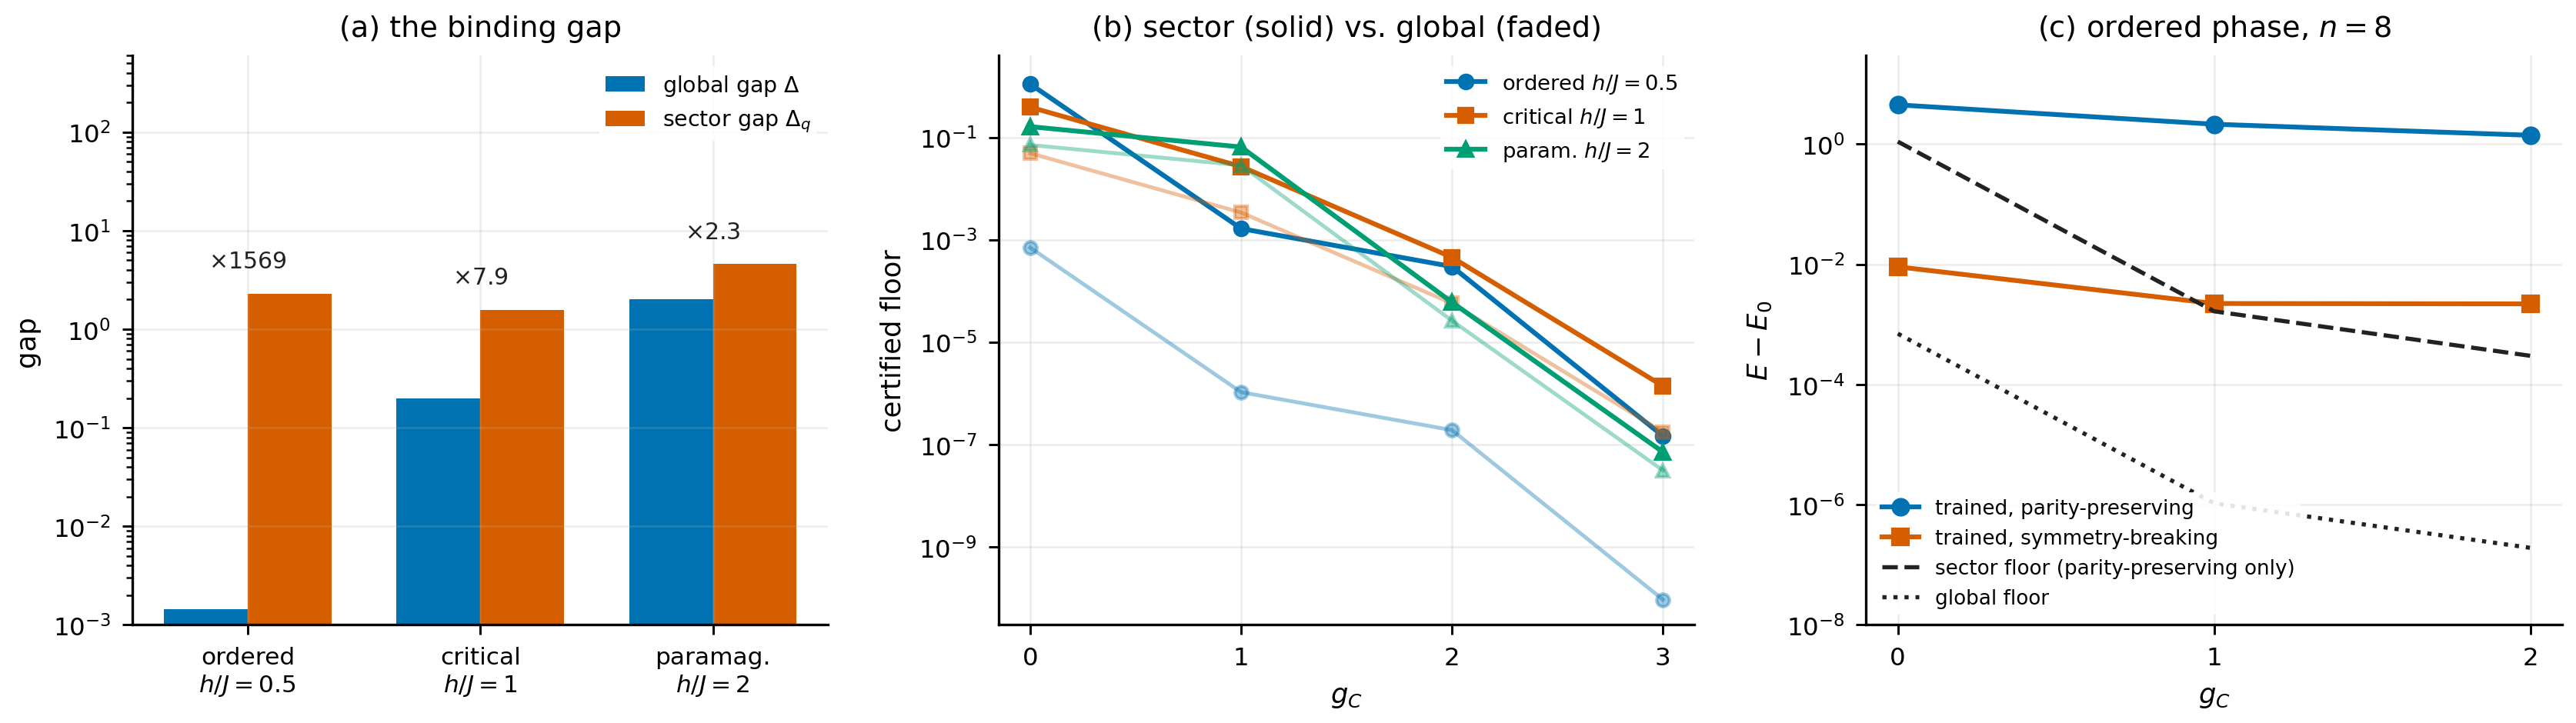
\includegraphics[width=\textwidth]{figures/sector.png}
  \caption{Sector-resolved certificate on the periodic TFIM at $n=8$.
  \emph{(a)} Global gap $\Delta$ versus $P=+1$ sector gap $\Delta_q$, annotated
  by their ratio.
  \emph{(b)} Certified floor versus $g_C$ for sector (solid) and global (faded)
  gaps.
  \emph{(c)} Ordered phase ($h/J=0.5$): trained errors for parity-preserving and
  symmetry-breaking circuits against both floors.}
  \label{fig:sector}
\end{figure*}

\Cref{tab:sector} and \Cref{fig:sector} compare the two families in all three
phases at $n=8$. In the ordered phase, symmetry produces the largest increase in
the certified floor: the global gap is much smaller than the accessible sector gap for the
parity-preserving circuit, and the sector floor at $g=0$ is $1.10$ rather than
$7.0\times10^{-4}$, a factor of $1569$. At the critical point, symmetry still
strengthens the certificate, but by a smaller factor ($\Delta_q/\Delta=7.9$). In the paramagnetic phase, the global and sector gaps
are already comparable, so the ratio is smaller, $\Delta_q/\Delta=2.3$.

Every parity-preserving run lies above its sector floor. The symmetry-breaking
HEA can reach energies below the sector floor---error $9.1\times10^{-3}$ at
$h/J=0.5$ and $g=0$, against a sector floor of $1.10$---because it is allowed to
leave the $P=+1$ sector and approach a nearly product, symmetry-broken member of
the low-energy doublet (\Cref{app:degenerate}).

Even for the parity-preserving circuit, a small sector floor does not guarantee
good performance. At $g=1$ in the ordered phase, two Schmidt components already
capture $\Lambda_C(2)=0.9993$ of the cat-like ground state, so the certified
floor is only $1.7\times10^{-3}$, while the trained error is $2.145$. The rank
condition is therefore necessary, not sufficient.

\section{Finite-size validation and large-system scaling}

\label{sec:scaling}

We compare the rank certificate with direct diagonalization and trained VQE on
small TFIM chains. We then use the exact free-fermion representation of the
open TFIM to evaluate the same quantities up to $n=128$, without many-body
truncation. Numerical details are given in \Cref{app:numerics}, together with two
further checks of the rank certificate: its dependence on gate scheduling, and
the roles of gap and fidelity deficit on the spin-$\tfrac12$ XXZ chain
(\Cref{app:checks}).

\subsection{Finite-size validation}

For the critical periodic TFIM ($J=h=1$) at $n=6$, the central-cut floor
decreases rapidly as cross-cut gates are added (\Cref{tab:single-cut}). With no crossing gate the floor is $6.02\times10^{-2}$.
One gate reduces it to $2.86\times10^{-3}$, two gates to $1.78\times10^{-5}$,
and at three gates the allowed Schmidt rank reaches the full dimension of the
smaller half, so the rank certificate becomes trivial. The certificate therefore becomes trivial after only three crossing gates in
this example.

\begin{table}[t]
\centering
\caption{Single-cut certificate on the critical periodic TFIM ($n=6$, central
cut, $E_0=-7.7274$, $\Delta=0.2633$).}
\label{tab:single-cut}
\begin{tabular}{rrcc}
\toprule
$g$ & $2^{g}$ & $\Lambda_C(2^{g})$ & floor\\
\midrule
$0$ & $1$ & $0.7712$ & $6.02\times10^{-2}$\\
$1$ & $2$ & $0.9891$ & $2.86\times10^{-3}$\\
$2$ & $4$ & $0.9999$ & $1.78\times10^{-5}$\\
$3$ & $8$ & $1.0000$ & ${\sim}10^{-16}$\\
\bottomrule
\end{tabular}
\end{table}

We also compare the certified energies with trained VQE energies on an $n=4$
critical periodic chain, using a three-layer HEA trained from $24$ restarts
(\Cref{tab:vqe}). Every trained energy lies above the corresponding
certified lower bound, with positive margins at $g=0$ and $g=1$. At $g=2$ the
rank certificate becomes trivial, and in this particular small example the
trained circuit also reaches the exact ground-state energy. The latter is an
empirical result, not a consequence of the certificate.

\begin{table}[t]
\centering
\caption{Trained VQE against the certified minimum energy
$E_0+\calC_\calA(H)$ on the critical periodic TFIM ($n=4$, $E_0=-5.2263$,
$\Delta=0.3978$; three-layer HEA, $24$ restarts). Columns give the certified
minimum energy, the best trained energy, and their difference.}
\label{tab:vqe}
{\small\setlength{\tabcolsep}{4pt}
\begin{tabular}{rccc}
\toprule
$g$ & certified min. & trained VQE & margin\\
\midrule
$0$ & $-5.1471$ & $-5.0000$ & $1.47\times10^{-1}$\\
$1$ & $-5.2246$ & $-5.0498$ & $1.75\times10^{-1}$\\
$2$ & $-5.2263$ & $-5.2263$ & ${\lesssim}10^{-12}$\\
\bottomrule
\end{tabular}}
\end{table}

\subsection{Scaling to 128 qubits}

To examine the size dependence, we evaluate the critical open TFIM up to
$n=128$. The TFIM is exactly reducible to free fermions,
allowing its gap and Schmidt spectrum to be obtained without storing the full
$2^n$-dimensional state (\Cref{app:numerics}); for $n\le12$ the free-fermion
values agree with exact diagonalization to at least nine digits.

The half-chain entropy follows the expected critical scaling
$S_{n/2}=\tfrac{c}{6}\ln(2n/\pi)+\mathrm{const}$: fitting the $n\ge32$ data gives
$c=0.515$, close to the exact Ising value
$c=1/2$~\cite{calabrese2004entanglement,sachdev2011quantum}
(\Cref{fig:scaling}a).

As the chain grows, the ground state becomes harder to approximate with Schmidt
rank two: the central-cut deficit $1-\Lambda_C(2)$ increases from
$1.09\times10^{-3}$ at $n=12$ to $1.57\times10^{-2}$ at $n=128$ (\Cref{tab:ff}).
At the same time, however, the critical spectral gap shrinks approximately as
$1/n$. These two effects largely cancel, and their product---the certified
energy floor at $g_C=1$---remains near $4\times10^{-4}$ over the entire size
range (\Cref{fig:scaling}b).

The target therefore becomes harder to approximate in fidelity without a
corresponding growth of the energy floor, because the critical gap closes at the
same time. Using the
parity-sector gap $\Delta_q$, which is close to $4\Delta$ here, raises the floor
by roughly another factor of four. Across the chain, the per-cut deficit has a smooth profile with its maximum at the central cut, suppressed by about two orders of magnitude
when a second crossing gate is added (\Cref{fig:scaling}c).

\begin{table}[t]
\centering
\caption{Exact free-fermion certificate inputs on the critical open TFIM.
Half-chain entropy $S_{n/2}$ is in nats; $\Delta_q$ is the gap in the $P=+1$
parity sector; $\Lambda_C$ and the floor are evaluated at the central cut.}
\label{tab:ff}
{\footnotesize\setlength{\tabcolsep}{2.8pt}
\begin{tabular}{rccccc}
\toprule
$n$ & $S_{n/2}$ & $\Delta$ & $\Delta_q$ & $1-\Lambda_C(2)$ & rank floor, $g{=}1$\\
\midrule
$12$  & $0.3965$ & $2.51{\times}10^{-1}$ & $1.00$ & $1.09{\times}10^{-3}$ & $2.74{\times}10^{-4}$\\
$16$  & $0.4234$ & $1.90{\times}10^{-1}$ & $0.760$ & $1.81{\times}10^{-3}$ & $3.45{\times}10^{-4}$\\
$24$  & $0.4602$ & $1.28{\times}10^{-1}$ & $0.512$ & $3.27{\times}10^{-3}$ & $4.19{\times}10^{-4}$\\
$32$  & $0.4857$ & $9.67{\times}10^{-2}$ & $0.386$ & $4.66{\times}10^{-3}$ & $4.50{\times}10^{-4}$\\
$48$  & $0.5211$ & $6.48{\times}10^{-2}$ & $0.259$ & $7.13{\times}10^{-3}$ & $4.62{\times}10^{-4}$\\
$64$  & $0.5458$ & $4.87{\times}10^{-2}$ & $0.195$ & $9.27{\times}10^{-3}$ & $4.51{\times}10^{-4}$\\
$96$  & $0.5804$ & $3.26{\times}10^{-2}$ & $0.130$ & $1.28{\times}10^{-2}$ & $4.17{\times}10^{-4}$\\
$128$ & $0.6048$ & $2.45{\times}10^{-2}$ & $0.098$ & $1.57{\times}10^{-2}$ & $3.84{\times}10^{-4}$\\
\bottomrule
\end{tabular}}
\end{table}

\begin{figure*}[t]
  \centering
  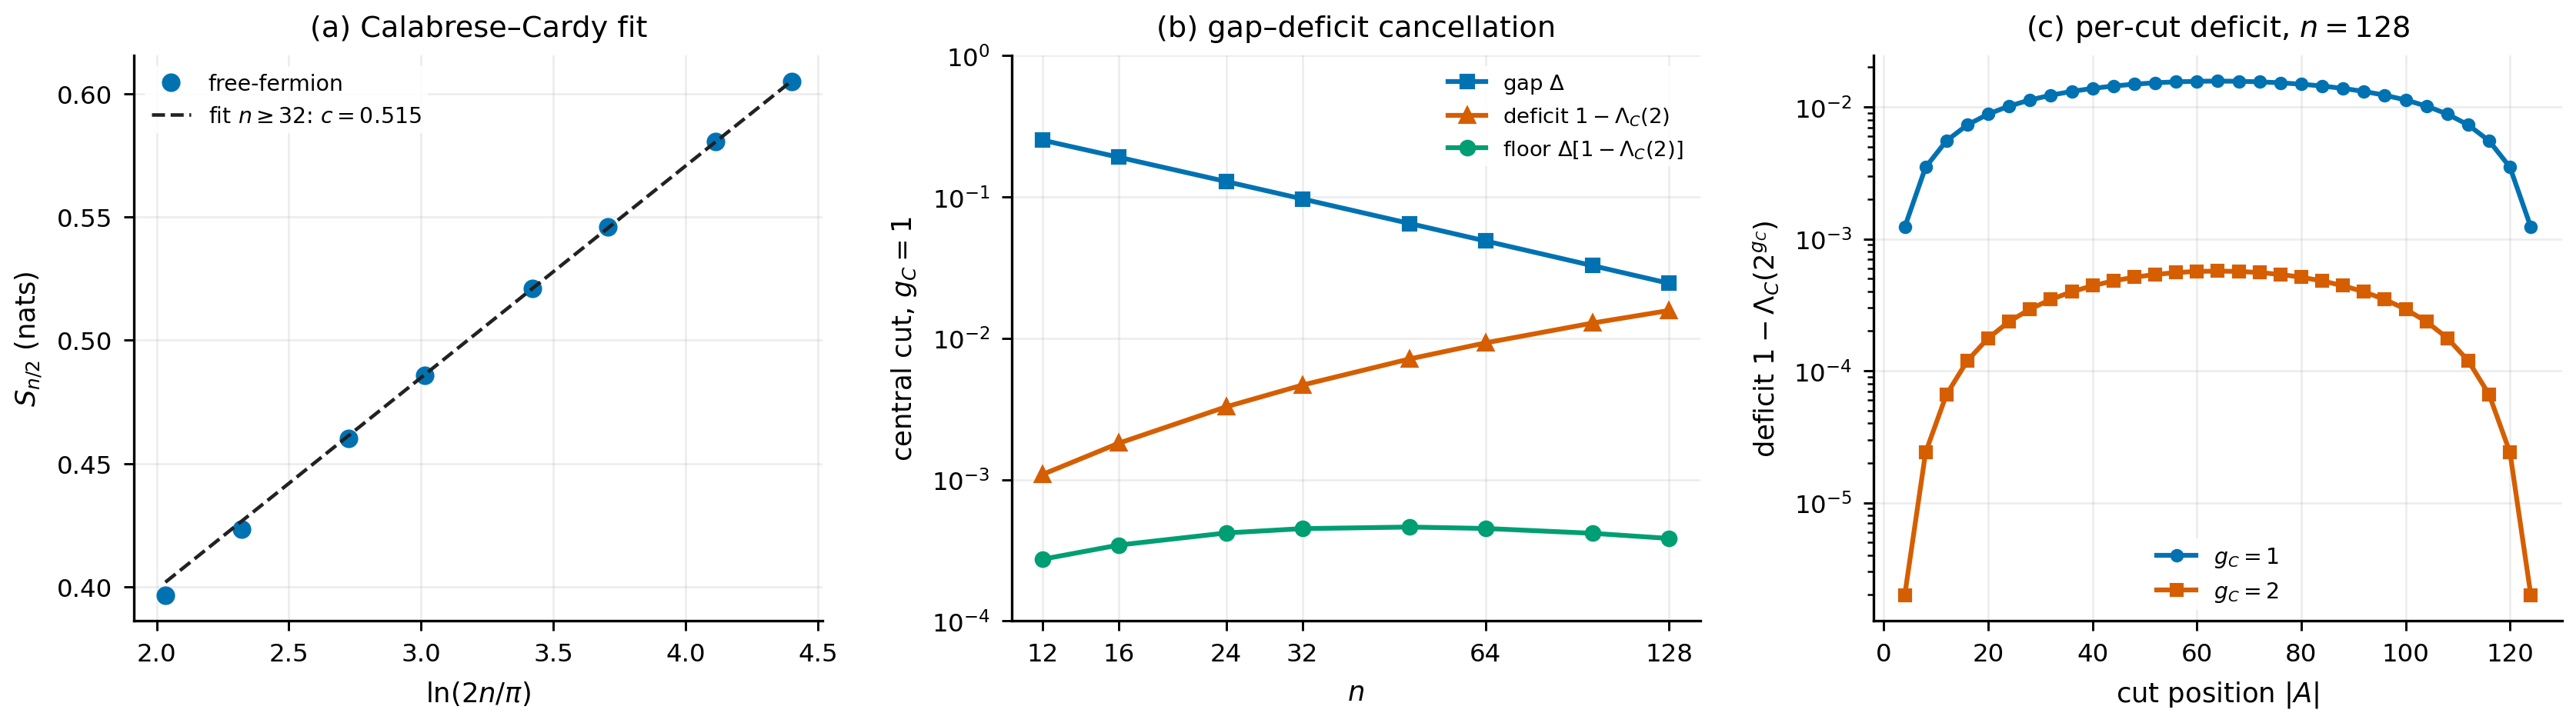
\includegraphics[width=\textwidth]{figures/scaling.png}
  \caption{Free-fermion evaluation on the critical open TFIM.
  \emph{(a)} Half-chain entropy (nats) versus $\ln(2n/\pi)$ to $n=128$, with a
  Calabrese--Cardy fit over $n\ge32$ giving $c=0.515$.
  \emph{(b)} Spectral gap $\Delta$, central-cut fidelity deficit
  $1-\Lambda_C(2)$, and their product, the certified floor at $g_C=1$, versus $n$: the deficit grows
  and the gap shrinks, leaving the floor nearly constant.
  \emph{(c)} Per-cut fidelity deficit $1-\Lambda_C(2^{g_C})$ across all cuts at
  $n=128$ for $g_C=1,2$.}
  \label{fig:scaling}
\end{figure*}

\section{Joint rank constraints across all cuts}
\label{sec:joint}

The basic certificate \eqref{eq:multi} checks one cut at a time. Yet a circuit
must satisfy its rank limits across every cut simultaneously. Imposing all cut-rank limits simultaneously can in principle strengthen the
single-cut floor. A state that is
individually allowed across each cut may still be impossible to realize while
respecting all of those rank limits at once; the single-cut certificate ignores
this compatibility between cuts.

Writing $\mathbf{R}=(R_0,\dots,R_{n-2})$ with $R_k=2^{g_{C_k}}$, define the
largest ground-state fidelity among states satisfying all cut-rank limits
simultaneously by
\begin{equation}
  \Lambda_{\mathrm{joint}}(\mathbf{R})
  :=\max_{\|\phi\|=1}|\braket{\psi_0}{\phi}|^2,\quad
  \rank_{C_k}(\phi)\le R_k\ \forall k.
\end{equation} Within the gap-and-fidelity framework, the strongest
energy floor implied jointly by these rank limits is
$\Delta[1-\Lambda_{\mathrm{joint}}(\mathbf{R})]$. If $\Lambda_{\mathrm{joint}}(\mathbf{R})$
is smaller than the tightest single-cut fidelity bound $\min_k\Lambda_{C_k}(R_k)$,
considering all cuts together strengthens the certificate.

Consider two independent Bell pairs on sites $(0,1)$ and $(2,3)$, and suppose
the circuit is not allowed to create entanglement across either of the two outer
cuts ($R_0=1$ and $R_2=1$, with $R_1=4$ on the central cut). Each outer cut
considered separately limits the squared overlap with the target to $1/2$.
Because both restrictions must hold at once, however, the maximum squared
overlap is $1/4$.

For general targets, we bound $\Lambda_{\mathrm{joint}}(\mathbf{R})$ and the
corresponding energy floor from both sides (\Cref{thm:joint} in
\Cref{app:joint}). Let $t_k:=1-\Lambda_{C_k}(R_k)$ denote
the single-cut Schmidt tail at cut $C_k$. The ordinary single-cut certificate
$\Delta\max_k t_k$ gives a lower bound on the joint floor. Analyzing disjoint
blocks of sites simultaneously sharpens that lower bound to a computable
multi-block quantity $\Delta[1-\Lambda_{\mathrm{MB}}(\mathbf{R})]$ (where MB
stands for ``multi-block''), which recovers the exact $1/4$ overlap in the
two-Bell-pair example above. Conversely, summing the single-cut tails gives an
upper bound:
\begin{align}
  \label{eq:jointfloor}
  \Delta\max_k t_k\ &\le\ \Delta\bigl[1-\Lambda_{\mathrm{MB}}(\mathbf{R})\bigr]
  \ \le\ \Delta\bigl[1-\Lambda_{\mathrm{joint}}(\mathbf{R})\bigr]\nonumber\\
  &\le\ \Delta\min\Bigl(1,\sum_k t_k\Bigr)\ \le\ m\,\Delta\max_k t_k ,
\end{align}
where $m:=|\{k:t_k>0\}|\le n-1$ is the number of cuts with a nonzero
single-cut tail. Within the gap-and-fidelity framework, using
all cut-rank constraints together can strengthen the single-cut certificate by
at most a factor $m$.

The analytical bounds leave a range in which the true joint floor must lie. For
small systems ($n\le12$) we narrow that range numerically by directly searching
for a matrix-product state (MPS) that satisfies the required bond dimensions
$R_k$ (\Cref{app:numerics}). Any normalized state found this way is feasible, so
its best squared overlap $F_{\mathrm{fit}}$ with $\ket{\psi_0}$ gives a lower
bound on $\Lambda_{\mathrm{joint}}(\mathbf{R})$, and therefore an upper bound
$\Delta(1-F_{\mathrm{fit}})$ on the joint energy floor.

\begin{figure}[t]
  \centering
  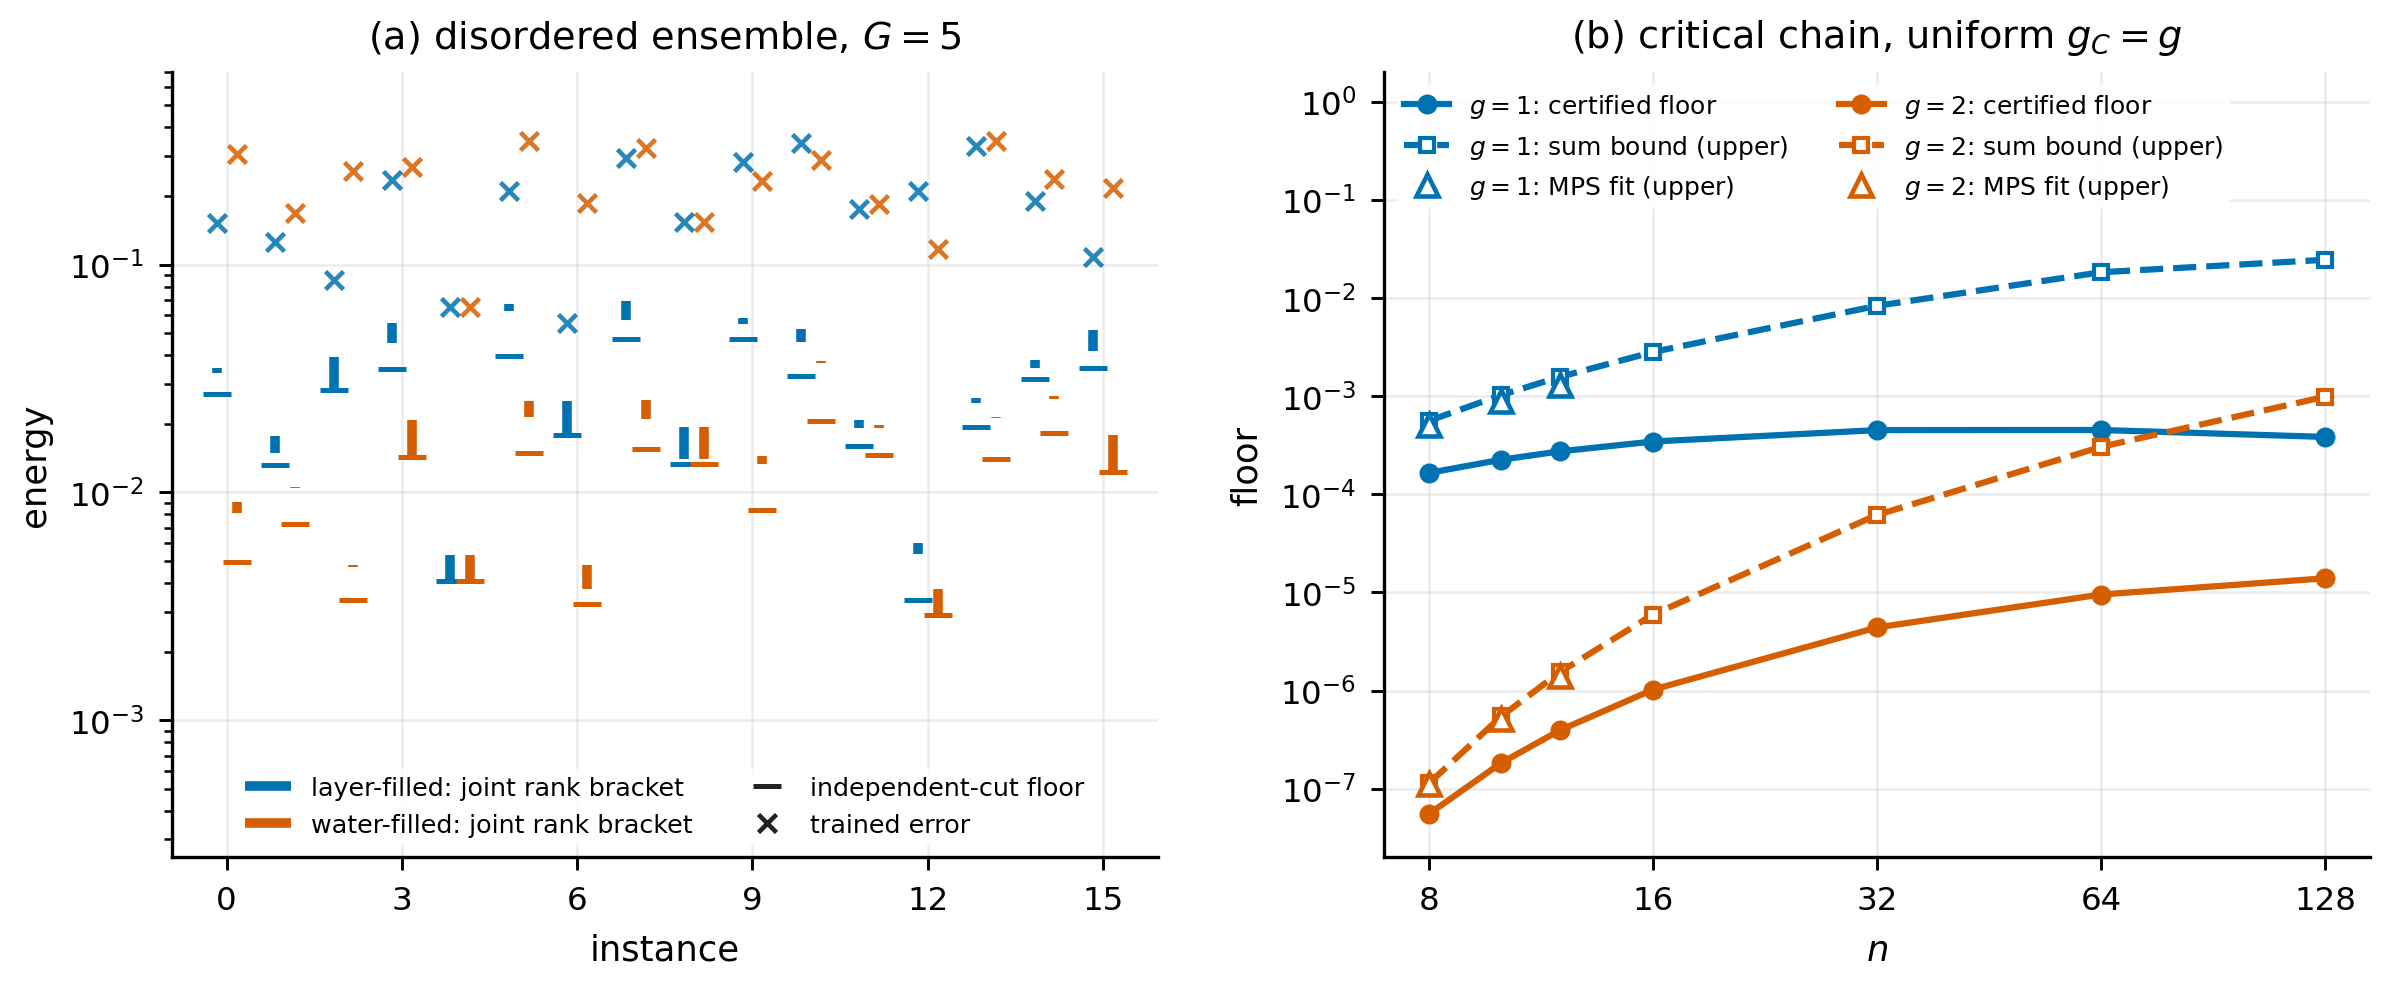
\includegraphics[width=\columnwidth]{figures/joint.png}
  \caption{Bracketing the optimal gap-based joint rank floor
  $\Delta(1-\Lambda_{\mathrm{joint}})$.
  \emph{(a)} Disordered TFIM ensemble at the disconnected budget $G=5$: vertical
  bars span the allowed range between the multi-block lower bound and the tighter
  of the MPS-fit and sum upper bounds; horizontal ticks mark the single-cut
  floor, and crosses show trained VQE errors.
  \emph{(b)} Critical open TFIM at uniform $g_C=g$: single-cut floor (equal here
  to the multi-block bound) compared with the MPS-fit upper bound ($n\le12$) and
  the analytical sum bound (to $n=128$).}
  \label{fig:joint}
\end{figure}

At the disconnected $G=5$ budget (\Cref{fig:joint}a), considering several cuts
together does raise the floor when empty bonds isolate parts of the chain, but
only modestly: the median increase over the single-cut floor is $1.22\times$
(maximum $1.79\times$), and combining the multi-block and MPS results bounds the true joint floor to within a median factor of $1.16$.

Once every bond has at least one entangler, the multi-block lower bound reduces
to the ordinary single-cut floor. On the uniform critical chain (\Cref{fig:joint}b), even the
numerical MPS upper bracket shows that the full joint treatment can raise the
rank floor by only $2$--$5\times$ for $n\le12$, while the analytical sum bound
extends to $n=128$, but its worst-case gap grows linearly with the number of
constrained cuts. The connected-circuit results below therefore cannot be attributed mainly to
treating the cuts independently.

\section{Testing rank-guided entangler allocation}
\label{sec:allocation}

We test the certificate as a rule for placing entangling gates. Suppose a nearest-neighbor chain can use only $G$ two-qubit
gates. If one cut has a larger certified floor than the others, placing the next
entangling gate there reduces the current bottleneck, and repeating this step
equalizes the bottlenecks across the chain. Writing $\mathbf{g}=(g_{C_0},\dots,g_{C_{n-2}})$ for the nonnegative integer
gate counts across the $n-1$ bonds and
$\varphi_k(g):=\Delta[1-\Lambda_{C_k}(2^g)]$ for the floor at cut $C_k$, this
min-max allocation problem is
\begin{equation}
  \label{eq:alloc}
  \calC^\star(G):=\min_{\mathbf{g}:\sum_k g_{C_k}\le G}\ \max_k\varphi_k(g_{C_k}).
\end{equation}
Equation~\eqref{eq:alloc} distributes $G$ gates so as to minimize the largest
remaining rank floor. For a nearest-neighbor chain, a water-filling rule solves
\eqref{eq:alloc} exactly: place each additional gate on a cut that currently has
the largest floor (\Cref{prop:waterfill} in \Cref{app:joint}).

\subsection{Disordered TFIM ensemble}
\label{sec:alloc-negative}

We test this design rule on $16$ disordered open $n=8$ TFIM chains ($7$ bonds),
$H=-\sum_{k=0}^{6}Z_kZ_{k+1}-\sum_{i=0}^{7}h_iX_i$, with $h_i$ drawn
log-uniformly from $[0.3,3]$. We use total gate budgets $G\in\{5,7,8,9,11\}$
and compare four layouts at each budget. The \emph{layer-filled} circuit is a uniform baseline. \emph{Water-filling} is
the layout chosen by \eqref{eq:alloc}. \emph{Connected water-filling} places at
least one gate on every bond before applying the same water-filling rule to the
remaining budget, which separates the effect of certificate-based placement from
the effect of leaving bonds empty. \emph{Connected random} imposes the same
one-gate-per-bond requirement but places the remaining gates at random. All
layouts at a fixed instance and budget use the same number of rotation parameters
and are trained from the same eight initialization seeds (\Cref{app:numerics}).

\begin{table}[t]
\centering
\caption{Disordered TFIM allocation ensemble ($n=8$ open, $16$ instances,
log-uniform $h_i\in[0.3,3]$, $8$ restarts, matched parameter counts). Here
$\Delta$med is the paired median of
$\mathrm{err}_{\mathrm{arm}}-\mathrm{err}_{\mathrm{layer}}$ (negative favors the
arm) with its $95\%$ bootstrap confidence interval (CI); ``win'' is the fraction
of instances beating the layer-filled baseline; ``floor'' is the median factor by
which the arm lowers the certified floor. Connected arms require $G\ge7$; at
$G=7$ all four arms assign one gate per bond and coincide.}
\label{tab:alloc}
{\scriptsize\setlength{\tabcolsep}{2.0pt}
\begin{tabular}{llccccc}
\toprule
$G$ & arm & med.\ err & $\Delta$med & $95\%$ CI & win & floor\\
\midrule
$5$ & water-filling      & $0.235$ & $+0.032$ & $[+0.000,+0.110]$ & $19\%$ & $2.1\times$\\
\midrule
$8$ & water-filling      & $0.050$ & $+0.002$ & $[-0.007,+0.015]$ & $38\%$ & $1.4\times$\\
$8$ & connected w.-fill  & $0.050$ & $+0.002$ & $[-0.007,+0.015]$ & $38\%$ & $1.4\times$\\
$8$ & connected random   & $0.055$ & $+0.000$ & $[-0.003,+0.007]$ & $31\%$ & $1.0\times$\\
\midrule
$9$ & water-filling      & $0.051$ & $+0.003$ & $[-0.001,+0.013]$ & $31\%$ & $2.4\times$\\
$9$ & connected w.-fill  & $0.051$ & $+0.003$ & $[-0.001,+0.013]$ & $31\%$ & $2.4\times$\\
$9$ & connected random   & $0.062$ & $+0.003$ & $[-0.005,+0.010]$ & $44\%$ & $1.0\times$\\
\midrule
$11$ & water-filling     & $0.110$ & $+0.014$ & $[+0.006,+0.066]$ & $6\%$  & $15.5\times$\\
$11$ & connected w.-fill & $0.110$ & $+0.014$ & $[+0.006,+0.066]$ & $6\%$  & $15.5\times$\\
$11$ & connected random  & $0.051$ & $-0.007$ & $[-0.022,+0.003]$ & $62\%$ & $1.0\times$\\
\bottomrule
\end{tabular}}
\end{table}

\begin{figure*}[t]
  \centering
  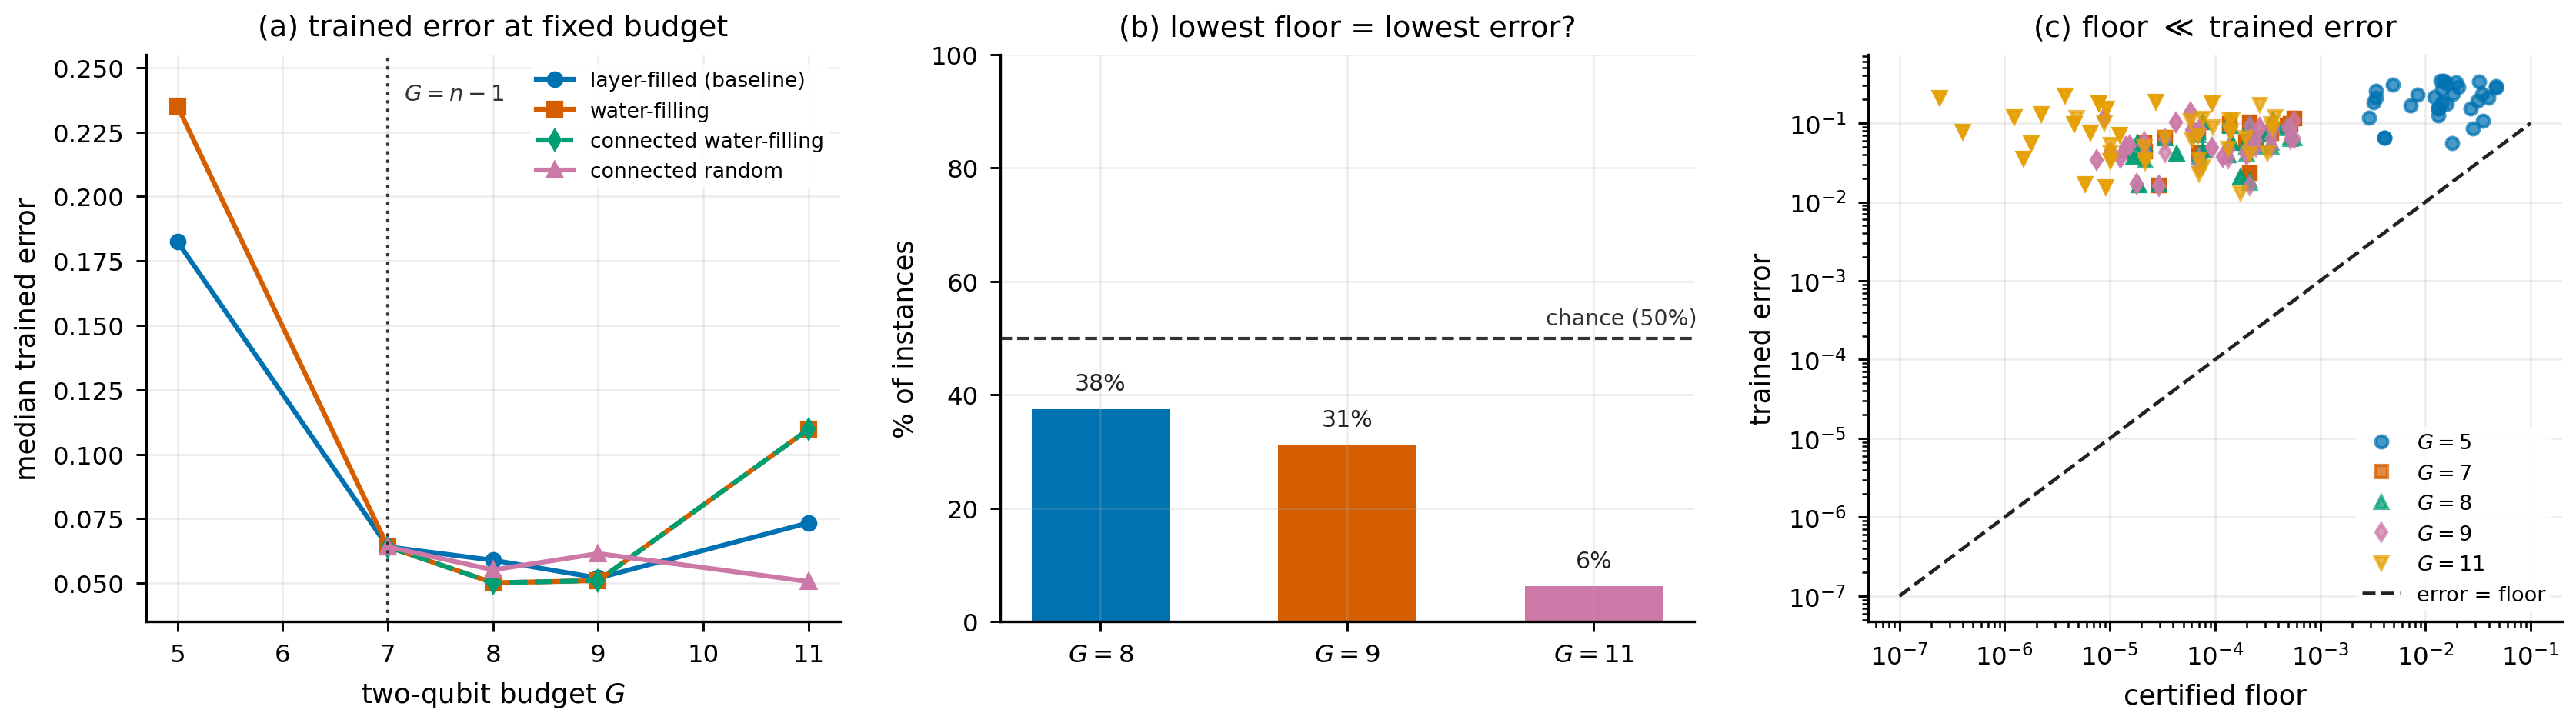
\includegraphics[width=\textwidth]{figures/allocation.png}
  \caption{Rank-guided allocation on the disordered open TFIM ensemble ($n=8$,
  $16$ instances, matched parameter counts).
  \emph{(a)} Median trained error versus budget $G$; connected and unconstrained
  water-filling coincide for all $G\ge n-1=7$ (dotted line).
  \emph{(b)} Percentage of instances in which the lowest-floor layout achieves
  lower trained error than the highest-floor layout (dashed line: $50\%$ chance).
  \emph{(c)} Trained error versus certified floor across all arms and instances;
  every point sits well above the equality line.}
  \label{fig:allocation}
\end{figure*}

Lowering the certified floor does not reliably lower the trained VQE error
(\Cref{tab:alloc} and \Cref{fig:allocation}). At $G=11$,
water-filling reduces the certified floor by a median factor of $15.5$, yet its
trained error is significantly \emph{higher} than the layer-filled baseline, and
it beats the baseline in only $1/16$ instances. At $G=8$ and $G=9$, we detect no statistically significant difference in
trained error between the layouts despite different certified floors, and at the disconnected budget $G=5$ water-filling also has the higher
median error. Within individual Hamiltonian instances, the lowest-floor layout beats the
highest-floor layout in only $38\%$, $31\%$, and $6\%$ of cases at $G=8$, $9$,
and $11$, respectively (\Cref{fig:allocation}b; full test statistics in
\Cref{app:numerics}).

\subsection{Limits of rank-guided allocation}

The result is not explained by disconnected circuits alone. For every
connected TFIM budget $G\ge7$, unconstrained and connected water-filling produce
the same gate allocation in all $16$ instances (\Cref{tab:alloc}), because
leaving any bond empty incurs a larger product-state penalty than the floors remaining after the other gates have been allocated. Enforcing connectivity therefore leaves the water-filling
layout unchanged (and a separate fragmentation control at $G=5$, reported in
\Cref{app:numerics}, shows no evidence of a bulk-disconnection penalty).

\begin{table}[t]
\centering
\caption{Scale separation between certified floors and trained errors across all
arms and instances of the disordered TFIM ensemble.}
\label{tab:active}
{\small\setlength{\tabcolsep}{5pt}
\begin{tabular}{rccc}
\toprule
$G$ & median floor & median trained err. & ratio\\
\midrule
$5$  & $1.47\times10^{-2}$ & $2.10\times10^{-1}$ & $14\times$\\
$7$  & $1.97\times10^{-4}$ & $6.41\times10^{-2}$ & $325\times$\\
$8$  & $1.34\times10^{-4}$ & $5.55\times10^{-2}$ & $414\times$\\
$9$  & $7.10\times10^{-5}$ & $5.32\times10^{-2}$ & $749\times$\\
$11$ & $1.02\times10^{-5}$ & $7.85\times10^{-2}$ & $7672\times$\\
\bottomrule
\end{tabular}}
\end{table}

The certified floors are also far below the trained errors. At every connected
TFIM budget, the certified floor is hundreds to thousands of times smaller than
the trained error, reaching a factor of $7672$ at $G=11$ (\Cref{tab:active}). A
floor this far below the observed error is too small to identify the source of
the trained error. Minimizing such a small lower bound need not reduce the
trained energy, and in these data concentrating additional gates on a few bonds
can increase it.

We also test whether the large separation comes from treating the cuts
independently. The joint bounds of \Cref{sec:joint} show that including all
cut-rank constraints does not close the floor--error gap within the
gap-and-fidelity framework. By \eqref{eq:jointfloor}, even
the largest gap-based floor consistent with all cut-rank constraints jointly
remains at least $35\times$ below every trained error across all instances and
arms at $G\ge7$ (and at $G=5$, where the joint floor is bracketed tightly in
\Cref{fig:joint}a, it orders the two layouts opposite to trained performance in
most instances; \Cref{app:numerics}). Within the gap-and-fidelity framework, the available rank information---not
merely the single-cut relaxation---is too weak to explain the observed errors in
this regime.

\subsection{Connected-budget control on a disordered Heisenberg chain}
\label{sec:heisenberg}

One possible explanation for the TFIM result is its large floor--error
separation, since the certified floors there lie far below the trained errors. We repeat the same $16$-instance, $n=8$ experiment on a disordered open
antiferromagnetic Heisenberg chain,
$H=\sum_{k=0}^{n-2}J_k(X_kX_{k+1}+Y_kY_{k+1}+Z_kZ_{k+1})$ with log-uniform
couplings $J_k\in[0.3,3]$, where the rank floor lies much closer to the trained
error. For positive couplings the ground state is a nondegenerate singlet by the
Lieb--Mattis theorem~\cite{lieb1962ordering}.

\begin{table}[t]
\centering
\caption{Connected-budget control on $16$ disordered open Heisenberg chains
($n=8$, log-uniform $J_k\in[0.3,3]$, $8$ restarts, matched parameter counts).
Columns match \Cref{tab:alloc}; at $G=7$ connected water-filling coincides
with the layer-filled baseline (``--'' indicates a tie on every instance).}
\label{tab:heisenberg}
{\scriptsize\setlength{\tabcolsep}{2.0pt}
\begin{tabular}{clccccc}
\toprule
$G$ & arm & med.\ err & $\Delta$med & $95\%$ CI & win & floor\\
\midrule
$7$  & water-filling     & $0.673$ & $+0.018$ & $[+0.008,+0.033]$ & $19\%$ & $1.5\times$\\
$7$  & connected w.-fill & $0.640$ & $+0.000$ & $[+0.000,+0.000]$ & --     & $1.0\times$\\
\midrule
$8$  & water-filling     & $0.709$ & $+0.009$ & $[-0.015,+0.031]$ & $44\%$ & $3.4\times$\\
$8$  & connected w.-fill & $0.640$ & $-0.000$ & $[-0.021,+0.019]$ & $50\%$ & $1.5\times$\\
$8$  & connected random  & $0.583$ & $+0.000$ & $[-0.002,+0.000]$ & $44\%$ & $1.0\times$\\
\midrule
$9$  & connected w.-fill & $0.582$ & $-0.011$ & $[-0.046,+0.000]$ & $62\%$ & $3.5\times$\\
$9$  & connected random  & $0.574$ & $-0.006$ & $[-0.056,+0.000]$ & $56\%$ & $1.0\times$\\
\midrule
$11$ & connected w.-fill & $0.622$ & $-0.012$ & $[-0.038,+0.039]$ & $56\%$ & $62.9\times$\\
$11$ & connected random  & $0.529$ & $-0.070$ & $[-0.132,-0.027]$ & $75\%$ & $1.2\times$\\
\bottomrule
\end{tabular}}
\end{table}

At $G=7$--$9$, the separation between the certified floor and trained error
is reduced from hundreds of times in the TFIM to $13$--$19\times$ (\Cref{tab:heisenberg}; additional per-arm ratios and test
statistics are in \Cref{app:numerics}). Despite this much smaller separation,
the layout with the lower rank floor still does not consistently achieve the
lower trained error: unconstrained water-filling trains worse than the baseline
at $G=7$ when it leaves weak bonds empty, and across $G=8,9,11$ the lowest-floor
layout wins roughly half of the within-instance comparisons, with no detected departure from a $50\%$ win rate. At $G=11$, connected water-filling lowers the rank floor by
$62.9\times$ without significantly improving the trained energy, whereas the
connected-random control gives the largest trained-energy improvement while
changing the floor by only $1.2\times$.

The TFIM joint-rank test addresses the independent-cut approximation, while the
Heisenberg test addresses the large floor--error separation. In the TFIM, considering all rank constraints jointly still leaves the certified floor well
below the trained-error scale. In the Heisenberg ensemble,
bringing the rank floor much closer to that scale still does not make floor
minimization a reliable design rule. The failure is therefore not explained
solely by independent-cut looseness or by the large floor--error separation in
the TFIM. We have
not tested two-dimensional layouts or chemistry-motivated noncontiguous
partitions, where both target Schmidt spectra and crossing-gate patterns differ.

\section{Orbital-ordering bottlenecks in Fermi--Hubbard}
\label{sec:hubbard}

The previous sections changed the circuit while keeping the target fixed. We
next keep the physical Hamiltonian fixed and change only the spin-orbital
ordering. Under the Jordan--Wigner mapping, the ordering of spin-orbitals
determines which physical correlations are separated by each contiguous cut of
the qubit register. Different orderings give unitarily equivalent qubit
encodings of the same physical Hamiltonian, so $E_0$ and $\Delta$ are unchanged;
what changes is the Schmidt spectrum seen across each qubit cut, so differences
in the certificate arise from the changed qubit ordering.

We compare two common orderings on a chain of $L$ spatial sites:
\emph{interleaved} ordering, $(1\uparrow,1\downarrow,2\uparrow,2\downarrow,\dots)$,
which pairs opposite spins on the same site, and \emph{spin-sector} ordering,
$(1\uparrow,\dots,L\uparrow,1\downarrow,\dots,L\downarrow)$, which groups all
spin-up orbitals before all spin-down orbitals. Both represent the same
Fermi--Hubbard Hamiltonian; only the qubit ordering differs.

\begin{figure}[t]
  \centering
  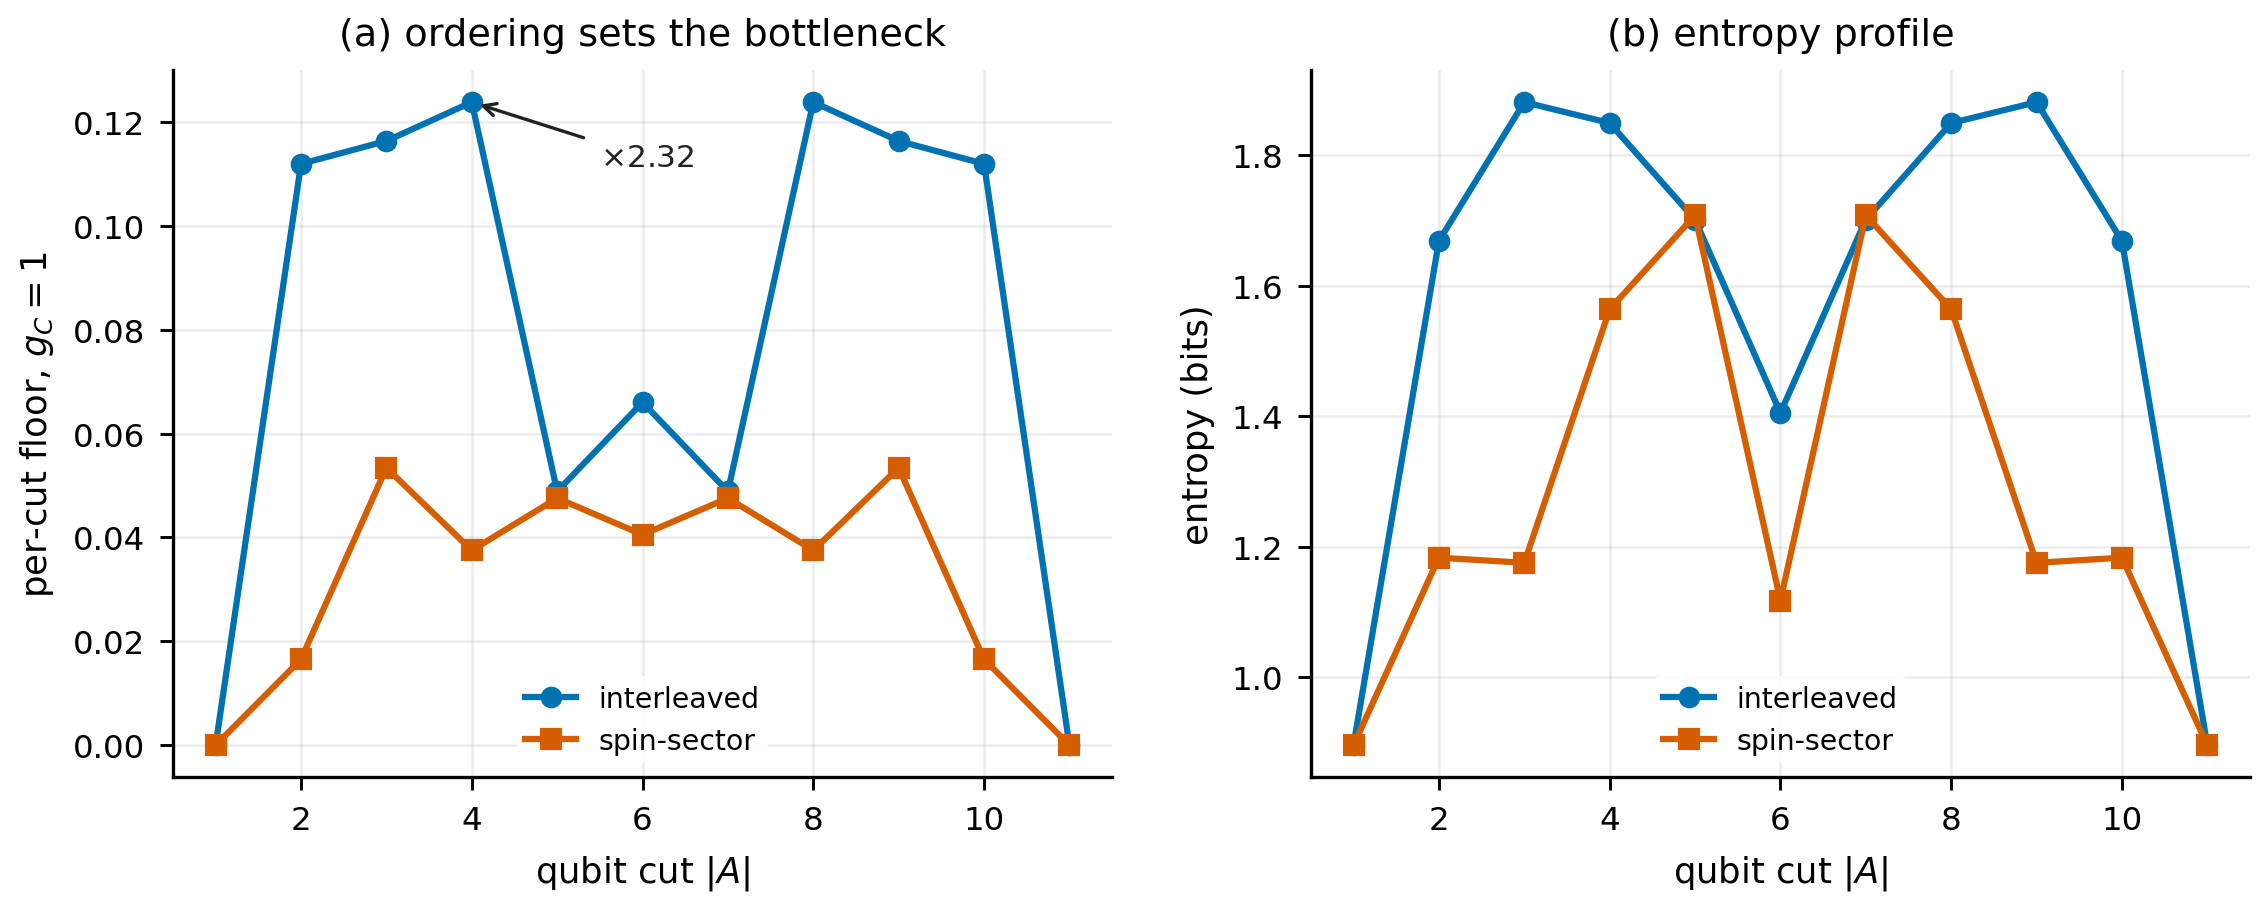
\includegraphics[width=\columnwidth]{figures/hubbard.png}
  \caption{Changing only the spin-orbital ordering changes where the
  entanglement bottleneck appears, with spin-sector ordering lowering the
  largest contiguous-cut floor by $2.32\times$. Data are for the open six-site
  ($12$-qubit) Fermi--Hubbard chain at $U/t=4$ (full $2^{12}$ space; global
  ground state in the $N=4$ sector with $E_0=-4.4221$ and $\Delta=0.3585$).
  \emph{(a)} Per-cut certified floor at $g_C=1$.
  \emph{(b)} Half-cut entanglement entropy profile (bits).}
  \label{fig:hubbard}
\end{figure}

We use the open six-site Fermi--Hubbard chain at $U/t=4$,
\begin{equation}
  H=-t\sum_{i,\sigma}\bigl(c^\dagger_{i\sigma}c_{i+1,\sigma}+\mathrm{h.c.}\bigr)
  +U\sum_i n_{i\uparrow}n_{i\downarrow},
\end{equation}
where $c^\dagger_{i\sigma}$ creates a fermion of spin
$\sigma\in\{\uparrow,\downarrow\}$ at site $i$,
$n_{i\sigma}=c^\dagger_{i\sigma}c_{i\sigma}$, and h.c.\ denotes the Hermitian
conjugate. Six spatial sites give $12$ qubits. We diagonalize the full $2^{12}$
Hilbert space rather than imposing a particle-number constraint, so
\Cref{thm:main} applies directly to particle-number-nonconserving HEA circuits;
the global ground state lies in the sector with total particle number
$N=\sum_{i,\sigma}n_{i\sigma}=4$, with $E_0=-4.4221$ and global gap
$\Delta=0.3585$ (\Cref{app:numerics}).

At one entangler per cut ($g_C=1$), the spin-sector ordering has a smaller
bottleneck than the interleaved ordering (\Cref{fig:hubbard}). Across
contiguous cuts, the largest certified floor falls from $0.1238$ (at cut $4$) to
$0.0534$ (at cut $3$), a factor of $2.32$. Because the physical Hamiltonian has
not changed, this difference comes entirely from how the qubit ordering
redistributes entanglement across the cuts available to the circuit. The same
ranking holds when all nontrivial bipartitions are checked rather than only
contiguous cuts, giving bottlenecks of $0.1329$ and $0.0716$ (\Cref{app:rank}).

For this single instance, trained VQE errors ($12$ shared-seed restarts of a
one-CNOT-per-bond HEA) are $1.788$ for the interleaved encoding and $1.080$ for
the spin-sector ordering, so they have the same ordering as the certified
floors. Both errors remain far above the floors, and this single-instance
agreement does not show that the floor generally predicts trained performance.

\section{Discussion}
\label{sec:discussion}

\subsection{What the certificate bounds}

The quantity bounded in this work is not the ground-state energy itself. It is
$\Estar$, the lowest energy reachable by a specified circuit architecture.
Standard VQE produces an upper bound on $E_0$ by training a circuit, whereas
dual-VQE methods~\cite{westerheim2024dual} train a dual program to lower-bound
$E_0$. Our certificate instead lower-bounds what a fixed circuit family can
achieve before its parameters are optimized (\Cref{tab:positioning}).

\begin{table}[t]
\centering
\caption{The three methods bound different quantities.}
\label{tab:positioning}
{\footnotesize\setlength{\tabcolsep}{3.6pt}
\begin{tabular}{lcccc}
\toprule
Method & bounds & direction & trains? & needs target data?\\
\midrule
VQE                                & $E_0$    & upper & yes & no\\
dual-VQE~\cite{westerheim2024dual} & $E_0$    & lower & yes & no\\
this work                          & $\Estar$ & lower & no  & yes\\
\bottomrule
\end{tabular}}
\end{table}

Unlike VQE and dual-VQE, the present bound requires the target Schmidt spectrum
and spectral gap as classical inputs.

\subsection{Applications of the certificates}

For shallow circuits, the rank certificate can rule out an architecture before
any training or quantum measurements are performed whenever the number of
crossing gates falls below the target's effective Schmidt-rank requirement
$\lceil\log_2 R_C(\varepsilon)\rceil$ (\Cref{tab:single-cut}).

The angle certificate applies particularly to weak, fixed, or hardware-limited
entanglers, such as fixed-step Trotter circuits, adiabatic schedules, native
fractional gates, or bounded-duration pulse schedules. In these settings gate
count alone gives every nonzero entangler full rank credit, whereas
\Cref{thm:angle} and \Cref{cor:pulse} retain information about how much cross-cut
interaction has actually been applied (\Cref{tab:angle_tfim}).

Among the examples studied here, the largest increase in the floor occurs in the
symmetry-resolved ordered TFIM. When the circuit
cannot leave a fixed symmetry sector, excitations in other sectors do not weaken
the energy bound, and replacing the global gap by the in-sector gap in
\eqref{eq:sectorfloor} can strengthen the certificate by orders of magnitude
(\Cref{tab:sector}).

The certificate can also compare different encodings of the same Hamiltonian.
Because $E_0$ and $\Delta$ are invariant under unitarily equivalent qubit
encodings, differences in the floor directly reflect how an encoding
redistributes entanglement across the circuit's cuts, as in the Fermi--Hubbard
ordering test (\Cref{sec:hubbard}).

The allocation experiments in \Cref{sec:allocation}, however, show that minimizing the rank floor does not reliably improve trained VQE
performance in the systems studied here.

\subsection{Limitations and open problems}

Evaluating the bounds requires target-state information, and computing
$\Lambda_C(R)$ exactly is difficult for generic large many-body systems. We
therefore evaluate the present bounds on benchmarks, small systems, integrable
models, and analytically tractable cases, rather than as a replacement for VQE on an unknown large system.
Upper-bounding $\Lambda_C(R)$ from properties of the Hamiltonian would avoid the
need to compute the target Schmidt spectrum.

The energy conversion uses only the first excited energy: the gap
inequality treats all excited-state weight as though it lies at $E_1$, so it can
be loose whenever inaccessible weight is pushed into higher excitations.
Incorporating energy variance or additional spectral information could tighten
this step, while near-degenerate manifolds without a separating symmetry require
certified outer bounds on subspace capacity (\Cref{app:degenerate}).

For larger systems we do not yet know the exact joint fidelity allowed by
all cut-rank constraints simultaneously. \Cref{thm:joint} bounds how much the
single-cut certificate can underestimate it, but an efficiently computable
tighter bound on the full joint rank capacity remains open for larger critical
chains.

All certificates here are noiseless. On hardware, applying more or
stronger entangling operations improves representational capacity while
accumulating physical error; combining the angle or pulse-area certificate with
a noise-induced energy floor~\cite{mishra2024classically} could capture this trade-off.

\section{Conclusion}
\label{sec:conclusion}

We developed lower bounds on the energy error that a fixed variational circuit
must have because of limits on the entanglement it can create across cuts of the
qubit register. The rank bound uses only the number of entangling gates
crossing each cut. It provides a rigorous way to rule out circuits that do not
have enough Schmidt-rank capacity to represent the target state.

In the one-dimensional examples studied here, the rank bound is informative only
at shallow cross-cut depth. Including the actual strength of partial entanglers
gives an angle-based certificate that remains informative after rank counting
has become trivial. Symmetry can strengthen the bound further: when a circuit
remains inside one symmetry sector, the relevant energy scale is the gap inside
that sector rather than the global gap.

The bounds can rule out circuits with insufficient cross-cut entangling capacity, but the allocation
experiments show that minimizing the rank floor does not reliably improve
circuit layouts in the systems studied here, even when the certified floor lies
much closer to the observed error. Open directions include Hamiltonian-only
bounds on Schmidt tails and extensions that combine the angle-budget floor with
hardware noise and interaction-time constraints.

\begin{acknowledgments}
The author thanks colleagues at the Information Networking Institute for helpful
discussions and comments on the manuscript.
\end{acknowledgments}

\paragraph*{Data and code availability.}
All Hamiltonian builders, certificate routines, the adjoint-gradient VQE
simulator, the free-fermion machinery, the MPS joint-capacity fitter, every
experiment script, and the figure generators are provided in the accompanying
code repository together with raw JSON and log outputs, requiring only NumPy,
SciPy, and Matplotlib.

\appendix
\onecolumngrid

\section{Rank certificate and informative window}
\label{app:rank}
\label{app:fidelity}

Among normalized states of Schmidt rank at most $R$ across cut $C$, the largest
overlap with $\ket{\psi_0}$ is obtained from its $R$ largest Schmidt components.

\paragraph{Proof of the fidelity ceiling.}
Represent $\ket{\psi_0}$ across cut $C$ in the computational basis by its
$2^{|A|}\times2^{|B|}$ coefficient matrix $M$, whose singular values are the
Schmidt coefficients $\lambda_1^{(C)}\ge\lambda_2^{(C)}\ge\cdots$ (padded with
zeros past $d_C$). Any normalized state $\ket{\phi}$ with $\rank_C(\phi)\le R$
has a coefficient matrix $X$ satisfying $\rank(X)\le R$ and Frobenius norm
$\|X\|_F=1$. Their inner product is $|\braket{\phi}{\psi_0}|=|\Tr(X^\dagger M)|$.
By von Neumann's trace inequality and Cauchy--Schwarz
(cf.\ Eckart--Young~\cite{eckart1936approximation}), writing
$\sigma_1(X)\ge\cdots\ge\sigma_R(X)$ for the singular values of $X$,
\begin{equation}
  |\braket{\phi}{\psi_0}|=|\Tr(X^\dagger M)|
  \ \le\ \sum_{i=1}^R\sigma_i(X)\,\lambda_i^{(C)}
  \ \le\ \Bigl(\sum_{i=1}^R\sigma_i(X)^2\Bigr)^{1/2}
         \Bigl(\sum_{i=1}^{\min(R,d_C)}\bigl(\lambda_i^{(C)}\bigr)^2\Bigr)^{1/2}
  =\sqrt{\Lambda_C(R)},
\end{equation}
so $|\braket{\phi}{\psi_0}|^2\le\Lambda_C(R)$, with equality for the normalized
truncation of $\ket{\psi_0}$ to its $R$ largest Schmidt components.
\hfill$\square$

\paragraph{Operator Schmidt rank and proof of \Cref{thm:main}.}
Any bipartite unitary across $C$ admits an operator Schmidt decomposition
$U=\sum_{\mu=1}^{\chi(U)}s_\mu A_\mu\otimes B_\mu$~\cite{nielsen2003quantum}, so
applying $U$ multiplies a state's Schmidt rank across $C$ by at most $\chi(U)$.
Nonlocal two-qubit gates satisfy $\chi(U)\in\{2,4\}$, with $\chi=2$ for gates
locally equivalent to controlled unitaries such as CNOT, CZ, and nontrivial
$e^{-i\theta Z\otimes Z}$ ($\chi=1$ when $\theta\in(\pi/2)\mathbb{Z}$), whereas
$i\mathrm{SWAP}$, $\sqrt{i\mathrm{SWAP}}$, and generic two-qubit gates have
$\chi=4$~\cite{vatan2004optimal,balakrishnan2010operator}. Starting from a
product state ($\rank_C=1$; or more generally initial rank $r_C^{(0)}$, for
which $2^{g_C}$ is replaced by $r_C^{(0)}\prod_j\chi(U_j)$), cut-local gates
leave $\rank_C$ unchanged and $g_C$ gates with $\chi\le2$ give
$\rank_C(\ket{\psi_\calA(\theta)})\le2^{g_C}$ regardless of gate ordering. Hence
$f:=|\braket{\psi_\calA(\theta)}{\psi_0}|^2\le\Lambda_C(2^{g_C})$. Expanding
$\ket{\psi_\calA(\theta)}$ in the eigenbasis of $H$ with non-degenerate ground
energy $E_0$ and gap $\Delta=E_1-E_0>0$ gives the variational gap inequality
\begin{equation}
  \label{eq:vargap}
  \bra{\psi_\calA(\theta)}H\ket{\psi_\calA(\theta)}-E_0
  \ \ge\ \Delta(1-f)\ \ge\ \Delta\bigl[1-\Lambda_C(2^{g_C})\bigr].
\end{equation}
Maximizing over cuts $C$ and taking $\min_\theta$ yields \eqref{eq:multi}.
\hfill$\square$

\begin{proposition}[Scope and informative window of the rank certificate]
\label{prop:window}
Fix a cut $C$ across which $\ket{\psi_0}$ has Schmidt rank $d_C$. Then:
(i) $\Delta[1-\Lambda_C(2^{g_C})]>0$ if and only if $2^{g_C}<d_C$;
(ii) the floor at $C$ vanishes whenever $g_C\ge\min(|A|,|B|)$ since
$d_C\le2^{\min(|A|,|B|)}$;
(iii) $\calC_\calA(H)=0$ if and only if the floor vanishes at every considered
cut; and
(iv) for any $\varepsilon>0$, with $R_C(\varepsilon)=\min\{R:1-\Lambda_C(R)\le\varepsilon\}$,
\begin{equation}
  g_C\ \ge\ g_C^\star(\varepsilon):=\bigl\lceil\log_2 R_C(\varepsilon)\bigr\rceil
  \quad\Longrightarrow\quad
  \Delta\bigl[1-\Lambda_C(2^{g_C})\bigr]\ \le\ \Delta\varepsilon .
\end{equation}
\end{proposition}

\begin{proof}
Statements (i)--(iv) follow immediately from monotonicity of $\Lambda_C(R)$, the
equivalence $\Lambda_C(R)=1\iff R\ge d_C$ together with
$d_C\le2^{\min(|A|,|B|)}$, nonnegativity of each
per-cut floor, and the definition of $R_C(\varepsilon)$.
\end{proof}

For an all-bond nearest-neighbor circuit with $p$ layers, $g_C=p$ on every
contiguous cut, so $p\ge\lfloor n/2\rfloor$ makes the rank certificate trivial on
all such cuts.

\paragraph{General bipartitions.}
In \eqref{eq:vargap} the cut $C$ can be an arbitrary subset $A\subset\{0,\dots,n-1\}$
with $g_C$ counting all entanglers straddling $A$ and $A^c$. On the $12$-qubit
Fermi--Hubbard instance of \Cref{sec:hubbard} ($g_{\text{bond}}=1$), maximizing
over all $2^{11}-1=2{,}047$ nontrivial bipartitions selects the interior interval
$\{3,\dots,8\}$ (crossed by two bonds, $g_C=2$) and raises the certified floor
from $0.1238$ to $0.1329$ (interleaved) and from $0.0534$ to $0.0716$
(spin-sector).

\section{Angle-budget theorem, tightness, and pulse-area limit}
\label{app:angle}

\subsection{Proof of the angle-budget theorem}

For normalized states, the Fubini--Study distance is
$d_{\mathrm{FS}}(\psi,\phi):=\arccos|\braket{\psi}{\phi}|\in[0,\pi/2]$. For a
bipartition $C$, let $\calS_K$ be the set of normalized states of Schmidt rank at
most $K$ across $C$, and define the Fubini--Study distance from $\ket{\psi}$ to
$\calS_K$ by
\begin{equation}
  \label{eq:dK}
  d_K(\psi):=\min_{\phi\in\calS_K}\arccos|\braket{\phi}{\psi}|
  =\arccos\sqrt{\Lambda_\psi(K)}\ \in[0,\pi/2],
\end{equation}
where $\Lambda_\psi(K)$ is the sum of the $K$ largest squared Schmidt
coefficients of $\ket{\psi}$ across $C$ (\Cref{app:fidelity}). Recall from
\eqref{eq:cost} that $\tilde\theta=\min_{k\in\mathbb{Z}}|\theta-k\pi/2|\in[0,\pi/4]$.

\begin{lemma}[Distance growth per entangler]
\label{lem:distance}
Let $P$ act on $A$ and $Q$ act on $B$, both Hermitian with $P^2=\mathbb{1}_A$
and $Q^2=\mathbb{1}_B$, and set $U=e^{-i\theta P\otimes Q}$. For every normalized
state $\ket{\psi}$ and every $K\ge1$,
\begin{equation}
  d_K(U\psi)\ \le\ d_K(\psi)+\tilde\theta .
\end{equation}
Moreover, cut-local unitaries leave $d_K$ invariant, and any cross-cut unitary of
operator Schmidt rank $\chi$ satisfies $d_{\chi K}(U\psi)\le d_K(\psi)$.
\end{lemma}

\begin{proof}
Choose $\ket{\phi}\in\calS_K$ attaining $d_K(\psi)$. By unitary invariance and
the Fubini--Study triangle inequality,
$d_K(U\psi)\le d_{\mathrm{FS}}(U\psi,U\phi)+d_K(U\phi)=d_K(\psi)+d_K(U\phi)$.
Since $U\ket{\phi}=\cos\theta\ket{\phi}-i\sin\theta\,(P\otimes Q)\ket{\phi}$ and
both $\ket{\phi}$ and $(P\otimes Q)\ket{\phi}$ belong to $\calS_K$, with
$x:=\bra{\phi}P\otimes Q\ket{\phi}\in\mathbb{R}$ we have
$|\bra{\phi}U\ket{\phi}|=|\cos\theta-ix\sin\theta|\ge|\cos\theta|$ and
$|\bra{\phi}(P\otimes Q)U\ket{\phi}|=|x\cos\theta-i\sin\theta|\ge|\sin\theta|$.
Thus $\cos d_K(U\phi)\ge\max\{|\cos\theta|,|\sin\theta|\}=\cos\tilde\theta$, so
$d_K(U\phi)\le\tilde\theta$. Cut-local unitaries preserve $\calS_K$, and an
operator-Schmidt-rank-$\chi$ gate maps $\calS_K$ into $\calS_{\chi K}$.
\end{proof}

The subset $J$ below contains gates controlled through their angle cost; the
remaining crossing gates are controlled only through their rank increase.

\begin{theorem}[Hybrid rank-and-angle certificate]
\label{thm:angle}
Let a circuit start from a product state across $C$ and apply $g$ cross-cut gates
$e^{-i\theta_j P_j\otimes Q_j}$ satisfying the hypotheses of \Cref{lem:distance},
interleaved with arbitrary cut-local unitaries. For any subset
$J\subseteq\{1,\dots,g\}$, set $\Theta_J:=\sum_{j\in J}\tilde\theta_j$,
$K:=2^{g-|J|}$, $R:=2^g$, and
$\gamma_C(K,R):=\arccos\sqrt{\Lambda_C(K)/\Lambda_C(R)}\in[0,\pi/2)$. Then the circuit output $\ket{\psi}$ obeys
\begin{equation}
  \label{eq:anglebound}
  |\braket{\psi_0}{\psi}|\ \le\ \sqrt{\Lambda_C(R)}\,
  \cos\bigl([\gamma_C(K,R)-\Theta_J]_+\bigr),
\end{equation}
and consequently
\begin{equation}
  \label{eq:anglefloor}
  E-E_0\ \ge\ \Delta\Bigl[1-\Lambda_C(R)\cos^2\bigl([\gamma_C(K,R)-\Theta_J]_+\bigr)\Bigr].
\end{equation}
For fixed $m=|J|$, the tightest overlap bound in \eqref{eq:anglebound} is
obtained by choosing the $m$ gates of smallest angle cost $\tilde\theta_j$. The
best overlap upper bound is therefore the minimum of \eqref{eq:anglebound} over
$m=0,\dots,g$; equivalently, the strongest certified energy floor is the maximum
of \eqref{eq:anglefloor} over $m=0,\dots,g$.
\end{theorem}

\begin{proof}
Track $(K,d_K)$ gate by gate from $\rank_C=1$ and $d_1=0$: each gate outside $J$
doubles the tracked rank without increasing distance, while each gate in $J$
increases distance by at most $\tilde\theta_j$ by \Cref{lem:distance}. The final
state has $\rank_C(\psi)\le R=2^g$ and $d_K(\psi)\le\Theta_J$. Writing $\mu_1\ge\mu_2\ge\cdots$
for the Schmidt coefficients of $\ket{\psi}$ across $C$ and setting
$b^2:=\sum_{i>K}\mu_i^2=\sin^2 d_K(\psi)$ with $b=\sin\beta$ and
$\beta=d_K(\psi)\le\min\{\Theta_J,\pi/2\}$, von Neumann's trace inequality and
Cauchy--Schwarz on indices $1\le i\le K$ and $K<i\le R$ give
\begin{equation}
  |\braket{\psi_0}{\psi}|\ \le\ \sum_{i=1}^R\lambda_i^{(C)}\mu_i
  \ \le\ \sqrt{1-b^2}\sqrt{\Lambda_C(K)}+b\sqrt{\Lambda_C(R)-\Lambda_C(K)}
  \ =\ \sqrt{\Lambda_C(R)}\cos\bigl(\gamma_C(K,R)-\beta\bigr).
\end{equation}
Because $\cos(\gamma_C-\beta)$ increases monotonically for $\beta\in[0,\gamma_C]$
and achieves its maximum $1$ at $\beta=\gamma_C$, replacing $\beta$ by
$\min\{\Theta_J,\gamma_C\}$ yields \eqref{eq:anglebound}, and \eqref{eq:vargap}
gives \eqref{eq:anglefloor}. Smaller $\Theta_J$ never weakens \eqref{eq:anglebound},
so for fixed $m=|J|$ sorting $\tilde\theta_j$ and taking the $m$ smallest costs
is optimal.
\end{proof}

\paragraph{Single-gate form, triangle bound, and general two-qubit gates.}
For $g=1$ and $J=\{1\}$, setting $s(\theta):=\sin\tilde\theta=\min\{|\sin\theta|,|\cos\theta|\}$
reduces \eqref{eq:anglebound} to
\begin{equation}
  \label{eq:OC}
  |\braket{\psi_0}{\psi}|\ \le\ \max_{0\le b\le s(\theta)}
  \Bigl[\sqrt{1-b^2}\sqrt{\Lambda_C(1)}+b\sqrt{\Lambda_C(2)-\Lambda_C(1)}\Bigr].
\end{equation}
Truncating each gate in $J$ to its leading operator term in Hilbert-space norm
gives the triangle bound
$|\braket{\psi_0}{\psi}|\le\sqrt{\Lambda_C(K)}+\sum_{j\in J}\sin\tilde\theta_j$,
and \eqref{eq:anglebound} is never weaker than this triangle bound: with
$b_\star:=\sin\min\{\Theta_J,\gamma_C(K,R)\}\in[0,1]$, its right side equals
$\sqrt{1-b_\star^2}\sqrt{\Lambda_C(K)}+b_\star\sqrt{\Lambda_C(R)-\Lambda_C(K)}\le\sqrt{\Lambda_C(K)}+b_\star$.
For $\Theta_J\le\pi/2$, $b_\star\le\sin\Theta_J\le\sum_{j\in J}\sin\tilde\theta_j$;
for $\Theta_J>\pi/2$, concavity of $\sin$ on $[0,\pi/4]$ gives
$\sum_{j\in J}\sin\tilde\theta_j\ge(2\sqrt{2}/\pi)\Theta_J>\sqrt{2}>1\ge b_\star$,
so the triangle bound already exceeds $1$. The two can coincide (for example,
when every cost in $J$ vanishes), but the angle bound can be strictly stronger, because angles add like distances whereas the triangle bound adds
amplitudes and becomes vacuous once
$\sum_{j\in J}\sin\tilde\theta_j\ge1-\sqrt{\Lambda_C(K)}$ (\Cref{tab:angle}).
Any two-qubit unitary across $C$ is locally equivalent to the canonical
form $e^{-i(aXX+bYY+cZZ)}$~\cite{kraus2001optimal}, a product of three commuting
involutive interactions, and therefore carries total angle cost at most
$\tilde a+\tilde b+\tilde c$ (for CNOT or CZ this cost is $\pi/4$, where the rank
choice $J=\varnothing$ is always at least as strong).

\subsection{When the angle bound is tight}
\label{app:tight}

Suppose the cross-cut gates are traceless Pauli-string interactions
$e^{-i\theta_j P_j\otimes Q_j}$ and arbitrary cut-local unitaries on $A$ and $B$
are permitted. Write $\mu_1\ge\mu_2$ for the target's top two Schmidt
coefficients across $C$.

\paragraph{One crossing gate ($g=1$).}
Choosing product inputs $\ket{\alpha}\ket{\beta}$ ranging from eigenstates of
$P_1$ (output rank $1$) to states with $\bra{\alpha}P_1\ket{\alpha}=\bra{\beta}Q_1\ket{\beta}=0$
(output Schmidt coefficients $|\cos\theta_1|,|\sin\theta_1|$) continuously
realizes every second Schmidt coefficient $b\in[0,s(\theta_1)]$. Subsequent
cut-local unitaries map the output Schmidt vectors onto the top two Schmidt
vectors of $\ket{\psi_0}$, attaining overlap $\sqrt{1-b^2}\mu_1+b\mu_2$ and
matching \eqref{eq:OC} at $b=\min\{s(\theta_1),\sin\gamma_C(1,2)\}$.

\paragraph{Rank-two targets in the aligned-angle regime ($d_C\le2$, $\Theta_C\le\pi/4$).}
When $d_C\le2$ and $\Theta_C=\sum_{j=1}^g\tilde\theta_j\le\pi/4$, $\Lambda_C(R)=1$
for all $R\ge2$, so \eqref{eq:anglebound} reduces to
$|\braket{\psi_0}{\psi}|\le\cos([\alpha_C-\Theta_C]_+)$ with
$\mu_1=\cos\alpha_C$ and $\mu_2=\sin\alpha_C$ ($\alpha_C\le\pi/4$). Because all
traceless Pauli strings on a given block are unitarily equivalent, cut-local
unitaries between gates can align every interaction to a common axis
$P_1\otimes Q_1$ and adjust signs and $\pi/2$ shifts so the $g$ gates compose to
$e^{-i\Theta_C P_1\otimes Q_1}$. Since $\Theta_C\le\pi/4$, the one-gate
construction prepares smaller Schmidt weight $\sin\min\{\Theta_C,\alpha_C\}$ and
aligns Schmidt bases, attaining $\cos([\alpha_C-\Theta_C]_+)$ exactly. 

Aligned gates also show why the product distribution
$\bigotimes_j(\cos^2\theta_j,\sin^2\theta_j)$ is not a valid general
majorization bound on the output Schmidt weights: two aligned small-angle gates
yield tail weight $\sin^2(2\theta)\approx4\theta^2$ rather than $2\theta^2$. For
general many-body targets and restricted single-qubit layers, cut-local unitaries
cannot always align many-body Schmidt bases, so \Cref{thm:angle} remains a valid
bound without being attained.

\subsection{Pulse-area limit}

\begin{corollary}[Continuous-time pulse-area bound]
\label{cor:pulse}
Let the control Hamiltonian
$H_{\mathrm{ctrl}}(t)=H_A(t)+H_B(t)+\sum_k J_k(t)P_k\otimes Q_k$ on
$\calH_A\otimes\calH_B$, with $H_A(t)$ acting on $A$, $H_B(t)$ acting on $B$,
piecewise-continuous couplings $J_k(t)$, and Hermitian involutions $P_k,Q_k$,
generate the evolution, and let $\ket{\psi(T)}$ evolve under it from a product
state across $C$ over $[0,T]$. Let $H_{\mathrm{tar}}$ denote the target
Hamiltonian (the $H$ of the main text), with nondegenerate ground state
$\ket{\psi_0}$, ground energy $E_0$, and gap $\Delta$. Then
$d_1(\psi(T))\le\Theta_C(T):=\sum_k\int_0^T|J_k(t)|\,dt$, so
\begin{equation}
  \bra{\psi(T)}H_{\mathrm{tar}}\ket{\psi(T)}-E_0\ \ge\ \Delta\,\sin^2\bigl([\alpha_C-\Theta_C(T)]_+\bigr).
\end{equation}
Reaching $|\braket{\psi_0}{\psi(T)}|^2\ge F$ therefore requires
$\Theta_C(T)\ge[\alpha_C-\arccos\sqrt{F}]_+$ across every cut, yielding the time
lower bound \eqref{eq:pulsetime} whenever $|J_k(t)|\le J_{k,\max}$.
\end{corollary}

\begin{proof}
Approximate the evolution generated by $H_{\mathrm{ctrl}}$ by $N$-step
first-order Trotter products alternating
cut-local evolutions with factors $e^{-i J_k(t_m)\delta t\,P_k\otimes Q_k}$
($\delta t=T/N$). For sufficiently large $N$, $|J_k(t_m)|\delta t\le\pi/4$, so
\Cref{lem:distance} bounds $d_1$ of the Trotter state by the Riemann sum
$\sum_{m,k}|J_k(t_m)|\delta t$. Taking $N\to\infty$, norm convergence of the
Trotter product and continuity of $d_1$ establish $d_1(\psi(T))\le\Theta_C(T)$,
and \eqref{eq:speedfloor} gives the energy and fidelity bounds. Since
$\int_0^T|J_k(t)|\,dt\le J_{k,\max}T$, dividing by $\sum_k J_{k,\max}$ (or
$J_{\max}$ for a single term) yields \eqref{eq:pulsetime}.
\end{proof}

\section{Symmetry-sector certificate}
\label{app:sector}

\begin{theorem}[Sector-resolved certificate]
\label{thm:sector}
Let $Q$ be a Hermitian symmetry with $[H,Q]=0$, and let $\calH_q$ be the
eigenspace of $Q$ with eigenvalue $q$. Assume:
(a) the initial state satisfies $\ket{\psi_{\mathrm{init}}}\in\calH_q$ and has
Schmidt rank $1$ across $C$;
(b) the circuit $\calA$ preserves $\calH_q$ for all parameter values $\theta$
(sufficiently, every gate commutes with $Q$, or each variational layer maps
$\calH_q$ to itself);
(c) cross-cut gates have operator Schmidt rank at most $2$, with $g_C$ crossing
cut $C$;
(d) the restriction $H|_{\calH_q}$ has a non-degenerate lowest eigenvalue
$E_{0,q}$ with eigenstate $\ket{\psi_{0,q}}$ and sector gap
$\Delta_q:=E_{1,q}-E_{0,q}>0$; and
(e) $\Lambda_{C,q}(R)$ is the rank-$R$ fidelity capacity of $\ket{\psi_{0,q}}$
across $C$.
Then for all $\theta$,
\begin{equation}
  \bra{\psi_\calA(\theta)}H\ket{\psi_\calA(\theta)}
  \ \ge\ E_{0,q}+\max_C\,\Delta_q\bigl[1-\Lambda_{C,q}(2^{g_C})\bigr].
\end{equation}
If the global ground state $\ket{\psi_0}$ lies in $\calH_q$, then $E_{0,q}=E_0$
and $\Lambda_{C,q}=\Lambda_C$.
\end{theorem}

\begin{proof}
By (a) and (b), $\ket{\psi_\calA(\theta)}\in\calH_q$ for all $\theta$. Expanding
$\ket{\psi_\calA(\theta)}$ in an eigenbasis of the Hermitian operator
$H|_{\calH_q}$ and using (d) gives
$\bra{\psi_\calA(\theta)}H\ket{\psi_\calA(\theta)}-E_{0,q}\ge\Delta_q(1-|\braket{\psi_\calA(\theta)}{\psi_{0,q}}|^2)$.
The state $\ket{\psi_{0,q}}$ belongs to $\calH=\calH_A\otimes\calH_B$ even when
$\calH_q$ does not factorize across $C$. Hence by (a), (c), and
\Cref{app:fidelity}, $\rank_C(\ket{\psi_\calA(\theta)})\le2^{g_C}$ and
$|\braket{\psi_\calA(\theta)}{\psi_{0,q}}|^2\le\Lambda_{C,q}(2^{g_C})$.
Maximizing over cuts $C$ completes the proof.
\end{proof}

\paragraph{Parity preservation vs.\ breaking in TFIM ans\"atze.}
For $P=\prod_{i=0}^{n-1}X_i$, $\ket{+}^{\otimes n}$ has $P=+1$, every
$R_x(\theta)=e^{-i\theta X_i/2}$ commutes with $P$, and $X_k X_{k+1}$ commutes
with $Z_k Z_{k+1}$, so $e^{-i\theta Z_k Z_{k+1}}$ commutes with $P$ as well; the
$R_x$+$ZZ$ ansatz therefore satisfies \Cref{thm:sector}(a)--(c).

The standard HEA does not preserve this sector. Its initial state
$\ket{0}^{\otimes n}$ is an equal superposition of $P=+1$ and $P=-1$, $R_z$ does
not commute with $P$ because $Z_i$ anticommutes with $X_i$, and CNOT does not
preserve $P$ either: conjugating $\mathrm{CNOT}_{c\to t}=\tfrac12(I+Z_c)\otimes I+\tfrac12(I-Z_c)\otimes X_t$
by $X_c X_t$ maps $Z_c\mapsto -Z_c$ and gives
$(X_c X_t)\,\mathrm{CNOT}_{c\to t}\,(X_c X_t)=\mathrm{CNOT}_{c\to t}(I_c\otimes X_t)\neq\mathrm{CNOT}_{c\to t}$,
so none of these elements preserves $P=+1$.

Number-conserving gates such as $i\mathrm{SWAP}$ or Givens rotations preserve
$U(1)$ particle number with $\chi=4$, so \Cref{thm:sector} applies to them with
$2^{g_C}$ replaced by $4^{g_C}$.

\paragraph{Growth of the ordered-phase enhancement.}
\Cref{tab:sectorscaling} lists the global and sector gaps of the periodic TFIM at
$h/J=0.5$ for $n=6$ to $12$. The global gap is the splitting between the two
opposite-parity states of the low-energy doublet and closes exponentially, while
the $P=+1$ sector gap approaches a constant, so the enhancement grows roughly as
$e^{0.73n}$.

\begin{table}[h]
\centering
\caption{Ordered-phase sector enhancement on the periodic TFIM at $h/J=0.5$;
$\Delta$ is the global gap and $\Delta_q$ the gap within the $P=+1$ sector. A fit
gives $\Delta_q/\Delta\sim e^{0.73n}$.}
\label{tab:sectorscaling}
{\small\setlength{\tabcolsep}{6pt}
\begin{tabular}{rccc}
\toprule
$n$ & $\Delta$ & $\Delta_q$ & $\Delta_q/\Delta$\\
\midrule
$6$  & $6.89\times10^{-3}$ & $2.479$ & $360$\\
$8$  & $1.46\times10^{-3}$ & $2.284$ & $1.57\times10^{3}$\\
$10$ & $3.21\times10^{-4}$ & $2.187$ & $6.82\times10^{3}$\\
$12$ & $7.25\times10^{-5}$ & $2.132$ & $2.94\times10^{4}$\\
\bottomrule
\end{tabular}}
\end{table}

\section{Joint rank constraints and water-filling allocation}
\label{app:joint}

The multi-block bound enforces several cut-rank constraints at once by
restricting the dimension of the target reduced state on disjoint site blocks.

\begin{theorem}[Two-sided bound on joint rank capacity]
\label{thm:joint}
Let $\ket{\psi_0}$ be a normalized state on an open $n$-qubit chain, let $R_k$
be the rank allowed across cut $C_k$ (after site $k\in\{0,\dots,n-2\}$), and set
$t_k:=1-\Lambda_{C_k}(R_k)$. For any contiguous site interval $I=[a,b)$, define
$r(I)$ as the product of $R_k$ over the chain cuts bounding $I$ ($R_{b-1}$ if
$a=0$, $R_{a-1}$ if $b=n$, and $R_{a-1}R_{b-1}$ if $0<a<b<n$). For any
collection $\mathcal{I}$ of disjoint intervals with union $U=\bigcup_{I\in\mathcal{I}}I$,
let $K(\mathcal{I}):=\prod_{I\in\mathcal{I}}r(I)$ and let $\sigma_K(\rho_U)$ be
the sum of the $K$ largest eigenvalues of $\rho_U=\Tr_{U^c}\ket{\psi_0}\bra{\psi_0}$.
Defining $\Lambda_{\mathrm{MB}}(\mathbf{R}):=\min_{\mathcal{I}}\sigma_{K(\mathcal{I})}(\rho_U)$,
we have
\begin{equation}
  \label{eq:jointthm}
  1-\sum_{k=0}^{n-2}t_k\ \le\ \Lambda_{\mathrm{joint}}(\mathbf{R})
  \ \le\ \Lambda_{\mathrm{MB}}(\mathbf{R})
  \ \le\ \min_k\Lambda_{C_k}(R_k),
\end{equation}
which multiplies by $\Delta$ to give \eqref{eq:jointfloor}, with $m:=|\{k:t_k>0\}|$.
\end{theorem}

\begin{proof}
\emph{Upper bounds ($\Lambda_{\mathrm{joint}}\le\Lambda_{\mathrm{MB}}\le\min_k\Lambda_{C_k}$).}
Take any normalized $\ket{\phi}$ with $\rank_{C_k}(\phi)\le R_k$ for all $k$, and
consider an interior block $I=[a,b)$. Let $S_L\subset\calH_{<a}$ ($\dim S_L\le R_{a-1}$)
be the left Schmidt support of $\ket{\phi}$ across $C_{a-1}$ and
$S_R\subset\calH_{\ge b}$ ($\dim S_R\le R_{b-1}$) be its right Schmidt support
across $C_{b-1}$. Because the projectors onto $S_L\otimes\calH_{\ge a}$ and
$\calH_{<b}\otimes S_R$ act on disjoint site sets, they commute, placing
$\ket{\phi}$ in $S_L\otimes\calH_I\otimes S_R$. Expanding in orthonormal bases of
$S_L$ and $S_R$ writes $\ket{\phi}=\sum_{\alpha=1}^{R_{a-1}}\sum_{\beta=1}^{R_{b-1}}\ket{l_\alpha}\ket{M_{\alpha\beta}}\ket{r_\beta}$,
so the reduced state of $\ket{\phi}$ on $I$ is supported on
$\mathrm{span}\{\ket{M_{\alpha\beta}}\}$ of dimension at most
$R_{a-1}R_{b-1}=r(I)$ (and similarly with one factor for boundary intervals).
Let $P_I$ be the orthogonal projector onto that support on $\calH_I$. For
disjoint intervals $\mathcal{I}$, $\Pi:=\bigotimes_{I\in\mathcal{I}}P_I\otimes\mathbb{1}_{U^c}$
is an orthogonal projector fixing $\ket{\phi}$, and $\Pi_U:=\bigotimes_{I\in\mathcal{I}}P_I$
has rank at most $K(\mathcal{I})$. Hence by Cauchy--Schwarz and Ky Fan's maximum
principle,
$|\braket{\psi_0}{\phi}|^2=|\bra{\psi_0}\Pi\ket{\phi}|^2\le\bra{\psi_0}\Pi\ket{\psi_0}=\Tr(\Pi_U\rho_U)\le\sigma_{K(\mathcal{I})}(\rho_U)$.
Minimizing over $\mathcal{I}$ proves $\Lambda_{\mathrm{joint}}\le\Lambda_{\mathrm{MB}}$,
and choosing the single prefix $\mathcal{I}=\{[0,k+1)\}$ gives $K=R_k$ and
$\sigma_{R_k}(\rho_{[0,k+1)})=\Lambda_{C_k}(R_k)$.

\emph{Lower bound ($1-\sum_k t_k\le\Lambda_{\mathrm{joint}}$).}
Sequential truncated singular value decomposition (SVD) of $\ket{\psi_0}$
across cuts $k=0,\dots,n-2$ produces
an unnormalized tensor-train vector $\ket{\chi}$ satisfying $\rank_{C_k}(\chi)\le R_k$
at every cut and $\|\psi_0-\chi\|^2\le\sum_k t_k$~\cite{oseledets2011tensor}. If
$\sum_k t_k\ge1$ the claim is immediate; otherwise $\chi\neq0$, and the Euclidean
distance from the unit vector $\ket{\psi_0}$ to the complex line spanned by
$\ket{\chi}$ is $\sin\vartheta=\sqrt{1-|\braket{\psi_0}{\chi/\|\chi\|}|^2}\le\|\psi_0-\chi\|$,
yielding $\Lambda_{\mathrm{joint}}(\mathbf{R})\ge|\braket{\psi_0}{\chi/\|\chi\|}|^2\ge1-\sum_k t_k$.
By definition of $m$, at most $m$ terms are nonzero, each bounded by
$\max_k t_k$.
\end{proof}

\begin{proposition}[Exact greedy water-filling on a one-dimensional chain]
\label{prop:waterfill}
For $\varphi_k(g)=\Delta[1-\Lambda_{C_k}(2^g)]$, define
$g_k^{\min}(\tau):=\min\{g\ge0:\varphi_k(g)\le\tau\}$ and $B(\tau):=\sum_k g_k^{\min}(\tau)$.
Then: (i) $\max_k\varphi_k(g_{C_k})\le\tau$ if and only if $g_{C_k}\ge g_k^{\min}(\tau)$
for all $k$; (ii) $\calC^\star(G)=\min\{\tau:B(\tau)\le G\}$; and (iii) starting from $g_{C_k}=0$ on every bond and performing $G$ increments,
each on a cut currently maximizing $\varphi_k(g_{C_k})$, attains
$\calC^\star(G)$ in $O(n+G\log n)$ time using a binary max-heap. For connected
water-filling ($G\ge n-1$), the same rule starts from $g_{C_k}=1$ on all $n-1$
bonds and performs the remaining $G-(n-1)$ increments; the argument below applies
verbatim to the constrained problem with $g_k^{\min}(\tau)$ replaced by
$\max\{1,g_k^{\min}(\tau)\}$.
\end{proposition}

\begin{proof}
Items (i) and (ii) follow directly from monotonicity of each $\varphi_k$. For
(iii), whenever the current greedy maximum exceeds $\tau^\star=\calC^\star(G)$,
the chosen cut $k$ has $\varphi_k(g_{C_k})>\tau^\star$ and hence
$g_{C_k}<g_k^{\min}(\tau^\star)$, meaning every optimal allocation must assign at
least one more gate to cut $k$. Greedy therefore never overspends $B(\tau^\star)\le G$
before reaching $\tau^\star$. Building the heap takes $O(n)$ and each of the $G$
updates takes $O(\log n)$.
\end{proof}

\paragraph{Two-Bell-pair example and general coupling graphs.}
In the four-qubit example of \Cref{sec:joint}---two Bell pairs on $(0,1)$ and
$(2,3)$ with allowed ranks $\mathbf{R}=(1,4,1)$---choosing the single interior
interval $\mathcal{I}=\{[1,3)\}$ gives $K(\mathcal{I})=R_0 R_2=1$, projecting the
middle two qubits onto a one-dimensional product support across both outer cuts
simultaneously. Since $\rho_{[1,3)}=\tfrac14\mathbb{1}_4$, $\sigma_1(\rho_{[1,3)})=1/4$,
so $\Lambda_{\mathrm{MB}}(1,4,1)=1/4=\Lambda_{\mathrm{joint}}(1,4,1)$, whereas
each single-cut bound gives $\min_k\Lambda_{C_k}(R_k)=1/2$. Regarding
\Cref{prop:waterfill}, exact separability relies on each nearest-neighbor bond
crossing a single contiguous cut; on general coupling graphs where a
non-adjacent gate crosses several cuts at once, allocation becomes a covering
problem for which independent water-filling is only a relaxation.

\section{Degenerate and low-energy subspaces}
\label{app:degenerate}
\label{sec:degenerate}

For a degenerate ground space, or when a near-degenerate low-energy manifold is
the target of interest, fidelity with a single eigenstate can be
uninformative. We therefore measure how much weight the circuit can place inside
the entire low-energy eigenspace.

Let $\mathcal{L}$ be an $H$-invariant spectral subspace containing $\ket{\psi_0}$
with orthogonal projector $P_{\mathrm{L}}$ ($[H,P_{\mathrm{L}}]=0$), set
$\Delta_{\mathrm{out}}:=E_{\min}(\mathcal{L}^\perp)-E_0$, and define the
subspace capacity
$\Lambda_C^{\mathrm{L}}(R):=\max\{\bra{\phi}P_{\mathrm{L}}\ket{\phi}:\|\phi\|=1,\ \rank_C(\phi)\le R\}$.

\begin{theorem}[Low-energy-subspace certificate]
\label{thm:degenerate}
Under the circuit assumptions of \Cref{thm:main}, for every $\theta$ and every
cut $C$,
$\bra{\psi_\calA(\theta)}H\ket{\psi_\calA(\theta)}\ge E_0+\Delta_{\mathrm{out}}[1-\Lambda_C^{\mathrm{L}}(2^{g_C})]$.
\end{theorem}

\begin{proof}
Decompose $\ket{\psi_\calA}=P_{\mathrm{L}}\ket{\psi_\calA}+(I-P_{\mathrm{L}})\ket{\psi_\calA}$.
Spectral invariance $[H,P_{\mathrm{L}}]=0$ eliminates the cross term, giving
$\bra{\psi_\calA}H\ket{\psi_\calA}\ge E_0\bra{\psi_\calA}P_{\mathrm{L}}\ket{\psi_\calA}+(E_0+\Delta_{\mathrm{out}})(1-\bra{\psi_\calA}P_{\mathrm{L}}\ket{\psi_\calA})=E_0+\Delta_{\mathrm{out}}(1-\bra{\psi_\calA}P_{\mathrm{L}}\ket{\psi_\calA})$.
Since $\rank_C(\psi_\calA)\le2^{g_C}$, $\bra{\psi_\calA}P_{\mathrm{L}}\ket{\psi_\calA}\le\Lambda_C^{\mathrm{L}}(2^{g_C})$.
\end{proof}

Applying \Cref{thm:degenerate} as a certified lower bound requires an exact value
or upper bound on $\Lambda_C^{\mathrm{L}}(R)$. In the ordered periodic TFIM at
$n=8$ ($h/J=0.5$), taking $\mathcal{L}=\mathrm{span}\{\ket{\psi_0},\ket{\psi_1}\}$
gives two cat-like eigenstates ($\Lambda_C^{(j)}(1)\approx0.5$), yet the
symmetry-broken superposition $(\ket{\psi_0}+\ket{\psi_1})/\sqrt{2}\in\mathcal{L}$
is nearly a product state with $\Lambda_C(1)=0.999$, bounding the doublet floor
above by $1.4\times10^{-3}$, consistent with the small $g=0$ HEA error in
\Cref{tab:sector}. Conversely, for
$\mathcal{L}=\mathrm{span}\{\ket{\psi_0},\dots,\ket{\psi_{m-1}}\}$, summing
individual capacities gives the outer bound,
\begin{equation}
  \label{eq:LamLub}
  \Lambda_C^{\mathrm{L}}(R)\ \le\ \min\Bigl\{1,\ \sum_{j=0}^{m-1}\Lambda_C^{(j)}(R)\Bigr\},
\end{equation}
which becomes trivial whenever the separate capacities sum to at least $1$ (as in
the ordered doublet where $0.518+0.518>1$); a tighter outer bound would need to account for the $m$ eigenstates jointly, and
a semidefinite relaxation is one possible approach.

\section{Numerical methods, approximate inputs, and additional checks}
\label{app:numerics}

\subsection{Conventions, approximate inputs, and simulation algorithms}

\paragraph{Entropy units.}
With Schmidt probabilities $p_i=(\lambda_i^{(C)})^2$, we report von Neumann
entropy in nats ($-\sum_i p_i\ln p_i$) whenever comparing prefactors with the
Calabrese--Cardy formula $S_{n/2}=\tfrac{c}{6}\ln(2n/\pi)+\mathrm{const}$ (fitting
bits would inflate $c$ by $1/\ln2\approx1.443$), and in bits ($-\sum_i p_i\log_2 p_i$)
for qualitative profiles, stating units in each caption.

\paragraph{What is computed directly and what is trained.}
Certificates never require training. For $n\le12$ we obtain $E_0$ and $\Delta$
by numerical diagonalization and obtain the Schmidt coefficients across each cut
by reshaping the ground-state vector to a $2^{|A|}\times2^{|B|}$ matrix and
computing its full SVD. Sector quantities use an
explicit block decomposition: conjugating by $W^{\otimes n}$, with $W$ the
single-qubit Hadamard gate, makes $P=\prod_iX_i$ diagonal with eigenvalue
$(-1)^{w}$, where $w$ is the Hamming weight (the number of 1s in the
computational-basis bit string); each parity block is diagonalized separately and
its eigenvectors are rotated back before Schmidt spectra are taken. For open TFIM
chains up to $n=128$ we use the exact free-fermion representation described
below. Trained VQE is used only to compare optimized energies with the analytical
bounds. All layout comparisons use shared random restart seeds and matched
parameter counts, except where parameter differences are tabulated explicitly
(\Cref{tab:hardware}); the parity ansatz was checked to give $\langle P\rangle=1$
to machine precision at random parameters.

\paragraph{Hardware-efficient ansatz.}
Unless specified otherwise, circuits start from $\ket{0}^{\otimes n}$. Each of
the $L_{\mathrm{lay}}$ layers applies $R_y$ followed by $R_z$ on every qubit and
then CNOTs on the bonds that are active in that layer. A final $R_yR_z$ layer
gives $2n(L_{\mathrm{lay}}+1)$ unbounded rotation parameters. Bond $k$ is active
in layer $l=0,\dots,L_{\mathrm{lay}}-1$ when $l<g_{C_k}$, with control on qubit
$k$ and target on qubit $k+1$. All circuits use
an open linear entangler layout on the $n-1$ nearest-neighbor bonds, with no
wrap-around entangler even when $H$ is periodic. The angle-budget tests
replace CNOT with fixed-angle $e^{-i\theta Z_kZ_{k+1}}$, and the parity-sector
tests start from $\ket{+}^{\otimes n}$ and use $R_x$ layers with trainable
$e^{-i\theta Z_kZ_{k+1}}$.

\paragraph{Propagation of approximate classical inputs.}
While all certificate inputs in this work are computed without many-body
truncation (via \texttt{numpy.linalg.eigh} or \texttt{scipy.sparse.linalg.eigsh} at tolerance
$10^{-12}$~\cite{virtanen2020scipy}, full SVDs, or free-fermion covariance matrices without many-body truncation), the bounds remain valid whenever $\Delta$ is replaced by a lower bound
$\widehat\Delta\le\Delta$ and $\Lambda_C(R)$ by an upper bound
$\widehat\Lambda_C(R)\ge\Lambda_C(R)$. Let $\rho_C=\Tr_B\ket{\psi_0}\bra{\psi_0}$ denote the exact reduced density
matrix on side $A$ of cut $C$, so that $\Lambda_C(R)$ is the sum of its $R$
largest eigenvalues, and let $\|\cdot\|_1$ denote the trace norm. A variational
MPS approximation does not automatically supply an upper bound on
$\Lambda_C(R)$; however, if an approximate reduced state $\widetilde\rho_C$
satisfies
$\tfrac12\|\rho_C-\widetilde\rho_C\|_1\le\delta_C$, then, writing $\widetilde\Lambda_C(R)$ for the sum of the $R$ largest
eigenvalues of $\widetilde\rho_C$,
$\widehat\Lambda_C(R):=\min\{1,\widetilde\Lambda_C(R)+\delta_C\}\ge\Lambda_C(R)$
by Ky Fan's variational characterization.

\paragraph{Adjoint-gradient VQE.}
We simulate circuits by exact statevector contraction and compute gradients via a
single reverse-mode adjoint sweep~\cite{luo2019adjoint}. Writing the circuit as
$\ket{\psi_M}=G_M\cdots G_1\ket{\psi_{\mathrm{init}}}$, we first run one forward
sweep to obtain $\ket{\psi_M}$ and set the terminal costate
$\ket{\lambda_M}=H\ket{\psi_M}$. Stepping backward from $k=M$ to $1$, each
single-qubit rotation $G_k=e^{-i\theta_k P/2}$ contributes partial derivative
$\partial E/\partial\theta_k=\mathrm{Im}\bra{\lambda_k}P\ket{\psi_k}$ (or
$2\,\mathrm{Im}\bra{\lambda_k}Z_jZ_{j+1}\ket{\psi_k}$ for $e^{-i\theta_k Z_jZ_{j+1}}$).
We then uncompute both states via $\ket{\psi_{k-1}}=G_k^\dagger\ket{\psi_k}$ and
$\ket{\lambda_{k-1}}=G_k^\dagger\ket{\lambda_k}$. With $N_p$ the number of variational parameters, obtaining the energy and all
$N_p$ derivatives therefore takes $O(1)$ circuit sweeps rather than $O(N_p)$.
Gradients were verified against central finite differences to
$5\times10^{-10}$, and parameters were optimized with the limited-memory
Broyden--Fletcher--Goldfarb--Shanno algorithm with bounds (L-BFGS-B; \texttt{ftol}$=10^{-13}$, \texttt{gtol}$=10^{-10}$).

\paragraph{Exact free-fermion spectra.}
In Majorana operators $a_{2j}=(\prod_{m<j}X_m)Z_j$ and
$a_{2j+1}=(\prod_{m<j}X_m)Y_j$, the open TFIM reads
$H=\tfrac{i}{4}\sum_{m,n}\Omega_{mn}a_m a_n$ with $\Omega_{2j,2j+1}=-2h$ and
$\Omega_{2j+1,2j+2}=-2J$.

A real Schur decomposition $\Omega=O\,\Omega'\,O^{T}$, with $O$ orthogonal and
$\Omega'$ block-diagonal, yields single-particle energies
$\varepsilon_1\le\varepsilon_2\le\cdots$ (giving $\Delta=\varepsilon_1$ and
$\Delta_q=\varepsilon_1+\varepsilon_2$) and the ground-state Majorana covariance
matrix $\Gamma_{mn}=\tfrac{i}{2}\langle[a_m,a_n]\rangle$.

Restricting $\Gamma$ to block $A$, the eigenvalues of
$i\Gamma_A$ appear in $\pm\nu_j$ pairs~\cite{peschel2003calculation,vidal2003entanglement};
retaining one member of each pair, we extract the $R$ largest reduced-state
eigenvalues $\prod_j(1\pm\nu_j)/2$ with a max-heap over sign flips. Against exact diagonalization at $n=8,10,12$,
the entropies agree to nine digits and the top-eight Schmidt probabilities to $2\times10^{-15}$.

\paragraph{Random-circuit validation of \Cref{lem:distance}.}
Across $600$ six-qubit circuits with random cuts, random product inputs, $1$--$4$
random-angle $ZZ$ gates interleaved with independent Haar-random block unitaries,
and all $2{,}019$ subset checks with $\Theta_J<\pi/2$, the bound
$\Lambda_\psi(K)\ge\cos^2\Theta_J$ held with maximum round-off discrepancy
$2.0\times10^{-15}$.

\paragraph{MPS joint-capacity fitting.}
For \Cref{sec:joint}, $\Lambda_{\mathrm{MB}}$ enumerates all $2^n-1$ nonempty
subsets $U$ (merged into maximal contiguous runs) for $n\le12$. To obtain $F_{\mathrm{fit}}$, we sweep alternating single-site MPS
updates while maintaining canonical form with QR (orthogonal--triangular) factorizations, from sequential-SVD and
random starts until overlap changes by $<10^{-13}$.

\paragraph{Allocation-ensemble protocol.}
In both $16$-instance allocation ensembles (\Cref{sec:allocation}), layer-filled
distributes the $G$ gates as evenly as possible from left to right ($G\bmod 7$
bonds receive $\lfloor G/7\rfloor+1$ gates). Connected random starts with one gate
on every bond and assigns the remaining gates randomly, with one draw per
instance. At a fixed instance and budget, all arms use the same layer count
$L_{\mathrm{lay}}=\max_{\mathrm{arms}}\max_k g_{C_k}$; bonds whose entanglers are
exhausted receive rotation-only layers. Water-filling ties are broken by the
lowest bond index. Exhaustive enumeration confirms that the TFIM floor-optimal
allocation is unique at $G=8,9,11$ for all $16$ instances. Paired medians use
$20{,}000$ bootstrap resamples, and significance tests use two-sided Wilcoxon
signed-rank tests.

\paragraph{TFIM allocation statistics.}
In the disordered TFIM ensemble (\Cref{tab:alloc}), Wilcoxon tests of
water-filling against the layer-filled baseline give $p=0.074$ at $G=5$,
$p=0.53$ at $G=8$, $p=0.13$ at $G=9$, and $p<0.001$ at $G=11$.

In the within-instance test comparing the distinct layouts with the lowest and highest
certified floors, exact two-sided sign tests against the $50\%$ null give
$p=0.45$ ($6/16$), $p=0.21$ ($5/16$), and $p=5.2\times10^{-4}$ ($1/16$) at
$G=8,9,11$.

At the disconnected budget $G=5$, fixing $G$ and varying only where
the two empty bonds fall shows that placing both zeros in the bulk (connected
blocks of sizes $3,2,3$) gives a slightly lower median trained error ($0.162$)
than placing them at the boundary ($0.183$, Wilcoxon $p=0.53$). In $13$ of the $14$ instances where layer-filling and water-filling differ at
$G=5$, their joint-floor brackets in \Cref{fig:joint}(a) are disjoint and place
layer-filling higher, yet water-filling has higher trained error in $10$ of
those $13$.

\paragraph{Heisenberg allocation statistics.}
In the disordered Heisenberg control (\Cref{tab:heisenberg}), overall median
error-to-floor ratios across all four arms are $13\times$, $15\times$,
$19\times$, and $369\times$ at $G=7,8,9,11$ (or $9.4\times$, $12.7\times$,
$16.8\times$, and $57.4\times$ when restricted to the three connected arms:
layer-filled, connected water-filling, and connected random).

Unconstrained water-filling leaves weakly coupled bonds empty in $15/16$ instances at $G=7$
and $12/16$ at $G=8$, and coincides with connected water-filling at $G\ge9$.
Within-instance lowest-floor win counts are $3/15$ non-tied instances at $G=7$
(20\%, sign-test $p=0.035$) and $7/16$ (44\%), $9/16$ (56\%), and $7/16$ (44\%)
at $G=8,9,11$ ($p=0.80$ in all three). At $G=11$, Wilcoxon tests against the
baseline give $p=0.98$ for connected water-filling ($\Delta\mathrm{med}=-0.012$)
versus $p=0.017$ for connected random ($\Delta\mathrm{med}=-0.070$).

\paragraph{Fermi--Hubbard sector check.}
On the $12$-qubit Fermi--Hubbard chain (\Cref{sec:hubbard}), explicit fixed-$N$
block diagonalization confirms that the global ground state ($E_0=-4.4221$) and
first excited state ($-4.0636$) both reside in $N=4$, whereas the lowest
half-filled ($N=6$) state lies at $-3.0926$.

\subsection{Additional checks: gate scheduling and the XXZ chain}
\label{app:checks}

\begin{table}[t]
\centering
\caption{Scheduling check on the critical periodic TFIM ($n=8$, $E_0=-10.2517$,
$\Delta=0.1970$; $12$ restarts). Here ``all-NN'' (all-nearest-neighbor) places an entangler on every bond in
each sweep, ``staggered'' alternates even and odd bonds, $L_{\mathrm{lay}}$ counts
entangling layers, and ``params.''\ is the rotation parameter count
$2n(L_{\mathrm{lay}}+1)$.}
\label{tab:hardware}
{\small\setlength{\tabcolsep}{5pt}
\begin{tabular}{lccccc}
\toprule
schedule & gates & $L_{\mathrm{lay}}$ & params. & floor & tr.\ err.\\
\midrule
all-NN, $2$ sweeps    & $14$ & $2$ & $48$ & $5.73\times10^{-5}$ & $0.1211$\\
staggered, $2$ rounds & $7$  & $2$ & $48$ & $3.40\times10^{-3}$ & $0.1508$\\
staggered, $4$ rounds & $14$ & $4$ & $80$ & $5.73\times10^{-5}$ & $0.1206$\\
\bottomrule
\end{tabular}}
\end{table}

\begin{figure}[t]
  \centering
  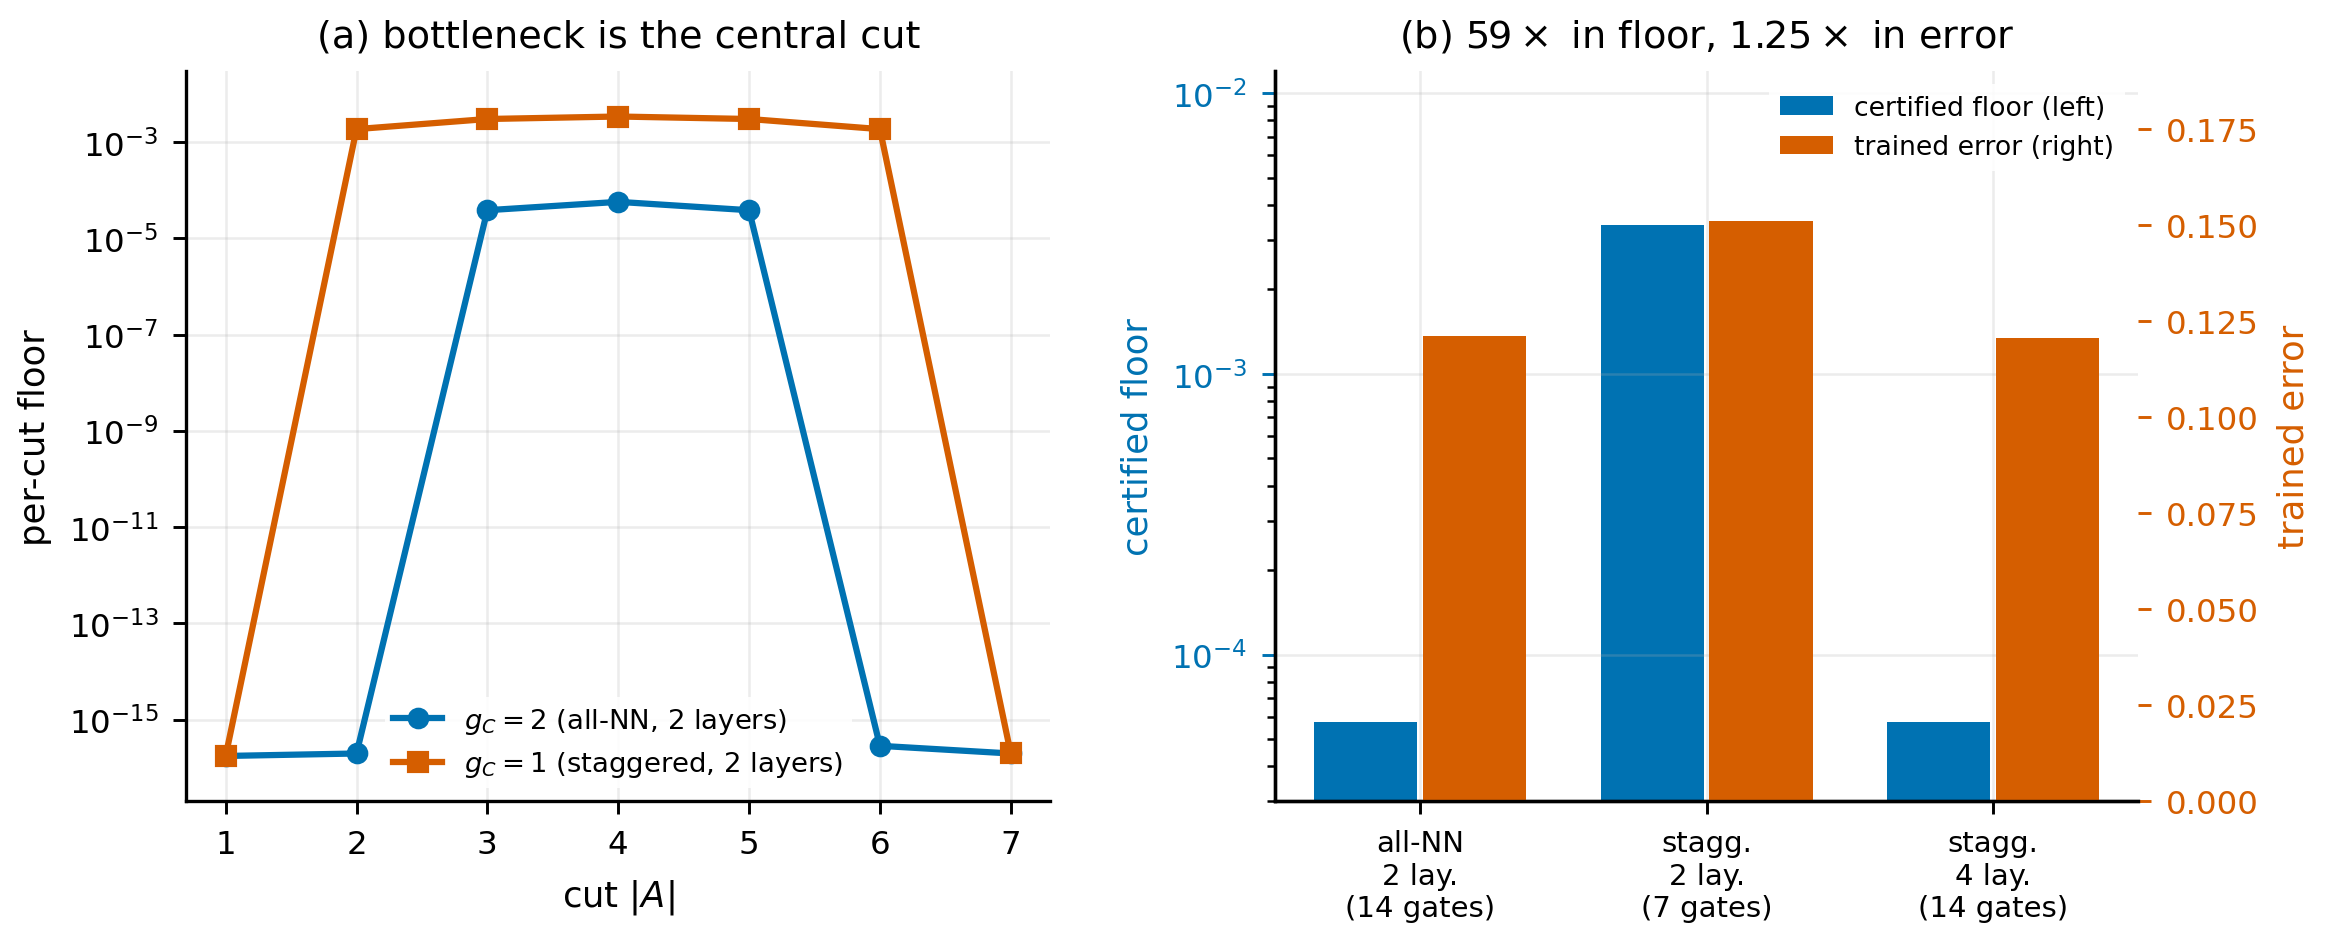
\includegraphics[width=0.58\textwidth]{figures/percut.png}
  \caption{\emph{(a)} Per-cut floor on the critical periodic TFIM ($n=8$) at
  $g_C=2$ (all-NN, $2$ layers) and $g_C=1$ (staggered, $2$ layers); outer cuts
  $1|7$ and $7|1$ vanish by dimension counting.
  \emph{(b)} Certified floor (left log axis) and trained error (right linear
  axis) for the three schedules of \Cref{tab:hardware}.}
  \label{fig:percut}
\end{figure}

\paragraph{Gate scheduling.}
Because \eqref{eq:multi} depends only on $g_C$, \Cref{tab:hardware} and
\Cref{fig:percut} compare an all-nearest-neighbor two-sweep schedule ($g_C=2$,
$14$ gates, $48$ parameters) against two-round ($g_C=1$, $7$ gates, $48$
parameters) and four-round ($g_C=2$, $14$ gates, $80$ parameters) even--odd
staggered schedules on the $n=8$ critical periodic TFIM. Halving $g_C$ from $2$
to $1$ raises the certified floor by $59\times$ while trained error rises by
$1.25\times$, whereas the two gate-matched $g_C=2$ schedules have the same certified floor and
nearly identical trained errors ($0.1211$ and $0.1206$), despite using $48$ and
$80$ parameters.

\begin{table}[t]
\centering
\caption{Spin-$\tfrac12$ XXZ chain ($n=8$, $J_{xy}=1$, periodic): half-chain entropy (bits),
spectral gap, single-gate capture $\Lambda_C(2)$, certified floor at $g_C=1$, and
trained VQE error ($12$ restarts).}
\label{tab:xxz}
{\small\setlength{\tabcolsep}{6pt}
\begin{tabular}{cccccc}
\toprule
$J_z$ & $S$ (bits) & $\Delta$ & $\Lambda_C(2)$ & floor & trained err.\\
\midrule
$0.0$ & $1.506$ & $0.398$ & $0.7975$ & $8.06\times10^{-2}$ & $0.555$\\
$0.5$ & $1.517$ & $1.045$ & $0.7742$ & $2.36\times10^{-1}$ & $0.969$\\
$1.0$ & $1.465$ & $0.518$ & $0.8699$ & $6.73\times10^{-2}$ & $0.592$\\
$2.0$ & $1.235$ & $0.123$ & $0.9627$ & $4.57\times10^{-3}$ & $0.212$\\
$4.0$ & $1.076$ & $0.018$ & $0.9916$ & $1.54\times10^{-4}$ & $0.076$\\
\bottomrule
\end{tabular}}
\end{table}

\paragraph{Both gap and fidelity deficit matter.}
On the periodic $n=8$ XXZ chain
$H=\tfrac{J_{xy}}{2}\sum(X_iX_{i+1}+Y_iY_{i+1})+J_z\sum Z_iZ_{i+1}$ at $J_{xy}=1$
(\Cref{tab:xxz}), the half-chain entropy is nearly unchanged between $J_z=0$
and the isotropic point $J_z=0.5$ ($1.506$ vs.\ $1.517$ bits). The finite-size
gap, however, grows from $0.398$ to $1.045$, so the certified floor rises from
$8.06\times10^{-2}$ to $2.36\times10^{-1}$. The trained VQE error also rises,
from $0.555$ to $0.969$.

Across all five
anisotropies, both entropy and the certified floor have Spearman correlation
$\rho=0.900$ with trained error, while the gap-weighted floor distinguishes the $J_z=0$ and $J_z=0.5$ cases in
magnitude, whereas their entropies are nearly identical.

\twocolumngrid
\bibliographystyle{apsrev4-2}
\bibliography{refs}

\end{document}
